\documentclass[12pt,a4paper]{report}
\usepackage[utf8x]{inputenc}
\usepackage[T1]{fontenc}
\usepackage{lmodern}
\usepackage{ucs}
\usepackage{amsmath}
\usepackage{amsfonts}
\usepackage{amssymb}
%\usepackage{fullpage}
\usepackage[french]{babel}
\usepackage{xcolor}
\usepackage[pdftex]{graphicx}
\usepackage{titlesec}
\usepackage{cite}
\usepackage{pdfpages}
\usepackage{listings}
\usepackage{url}
\usepackage{rotating}
\usepackage[top=2cm,bottom=2.5cm,left=2.5cm]{geometry}

%%%%%%%%%%%%%%%%%encadrementdes chapitres%%%%%%%%%%%%%%%%%%%%%%%
\titleformat{\chapter} % commande de sectionnement affectée
[frame] % une des formes prédéfinies
{\itshape} % format appliqué au titre dans son ensemble
{\filright\small\enspace Chapitre \thechapter\enspace} % format du « n° » du titre
{8pt} % distance (horiz. ou vert.) entre le n° et le texte du titre
{\Large\bfseries\filcenter} % format appliqué au texte du titre
%%%%%%%%%%%%%%%%%%%%%%%%%%%%%%%%%%%%%%%%%%%%%%%%%%%%%%%%%%%%%%%%
\newcommand{\HRule}{\rule{\linewidth}{0.5mm}}
\title{Rapport Projet de programmation}
%\author{Charlotte \textsc{Herice}\\ Typhaine \textsc{Paysan-Lafosse}\\ Thomas \textsc{Faux}\\ Joris \textsx{Sansen}}
% Commenté car provoque une erreur lors de la compilation
\begin{document}
%\maketitle
%\documentclass[10pt,a4paper]{report}
%\usepackage[utf8x]{inputenc}
%\usepackage{ucs}
%\usepackage{amsmath}
%\usepackage{amsfonts}
%\usepackage{amssymb}
%\usepackage{fullpage}
%\usepackage[french]{babel}
%\usepackage{xcolor}
%\usepackage{graphicx}
%\newcommand{\HRule}{\rule{\linewidth}{0.5mm}}
%\begin{document}

\begin{titlepage}

\begin{center}


% Upper part of the page

\includegraphics[width=0.15\textwidth]{logounibdx.png}\\[1cm]

\textsc{\LARGE Université de Bordeaux}\\[1.5cm]
\vspace*{0.5cm}
%\textsc{\Large Projet Tutoré}\\[0.5cm]
\textsc{\Large Initiation à la Recherche\\\ et/ou Développement}\\[0.5cm]
%\textsc{\Large Development Project}\\[0.5cm]

\vspace*{1cm}

% Title
\HRule \\[0.3cm]
{ \begin{Huge}
\bfseries Rapport du projet de programmation :
\end{Huge} \\ \begin{huge}
Développement d'un utilitaire de sélection de particules observées au microscope électronique
\end{huge}}\\[0.3cm]

\HRule \\[1.3cm]
% Author and supervisor
\begin{minipage}{0.4\textwidth}
\begin{center} \large
%\emph{Author:}\\
Thomas \textsc{Faux}\\
Charlotte \textsc{Héricé}\\
Typhaine \textsc{Paysan-Lafosse}\\
Joris \textsc{Sansen}\\
\end{center}
\end{minipage}
\begin{minipage}{0.4\textwidth}
\begin{flushright} \large
%\emph{Supervisor:} \\
M. Jean-Christophe\textsc{Taveau}
\end{flushright}
\end{minipage}

\vfill

\begin{center}
2011-2012
\end{center}
% Bottom of the page

\includegraphics[width=0.4\textwidth]{./banniere_cbmn.png}\\[1cm]
CBMN - UMR 5248 \\
B8 AVENUE DES FACULTÉS \\
F-33402 TALENCE CEDEX \\

%{\large \today}

\end{center}

\end{titlepage}
%\end{document}
\newcommand{\cme}{cryo-MET}
\newcommand{\me}{MET}
\newcommand{\java}{Java~{\tiny \texttrademark}}
\newcommand{\js}{JavaScript}
\newcommand{\imj}{ImageJ}
%\renewcommand{\thefigure}{\arabic{figure}}

\begin{abstract}
\paragraph*{}
Dans le cadre des recherches de l'équipe ACMPC (Architecture des Complexes Membranaires et Processus Cellulaires) de l'unité mixte de recherche CNRS CBMN (Chimie et Biologie des Membranes et Nanoobjets), il est fréquent d'avoir à piquer manuellement un grand nombre de particules (complexes protéiques ou chimiques) sur des micrographies de microscopie électronique. Celles-ci sont ensuite traitées avec des outils statistiques en vue de calculer des images moyennes ou des reconstructions 3D (3 Dimensions). Pour cela, le logiciel \imj ~est couramment utilisé pour cette étape préliminaire, mais il ne dispose d'aucun outil automatique adapté pour traiter une grande quantité de données.
\paragraph*{}
L'objectif de notre projet a donc été de pallier à ce manque en créant un plugin pour ce logiciel. \imj ~étant implémenté en \java , nous avons créé une interface facile à utiliser en suivant ce langage. A l'heure actuelle, trois méthodes de sélection de particules (piquage) ainsi qu'un outil de découpage (\textit{crop} en anglais) de ces objets ont été implémenté.
\paragraph*{}
Ce plugin, nommé \emph{Pick\_EM} a également été créé dans le but de réunir dans un même outils plusieurs algorithmes, chacun ayant une sensibilité différente en fonction des cibles et de la qualité des images. Le code suit donc les règles de la programmation orientée objet afin de faciliter l'insertion d'une nouvelle méthode de piquage.

%\paragraph*{} Ce rapport traite de l'organisation globale du programme, de sa conception et de sa réalisation, expliquant les choix d'implémentation, 

%Le contexte de ce projet est l'étude de morphologies de virus ou de patchs de virus observés au microscope électronique (ME) dans le cadre d'une prestation de services avec une société pharmaceutique. Le projet consiste en le développement d'un utilitaire qui sélectionne automatiquement les particules virales et les protéines membranaires dans les images issues de \cme. Cet utilitaire se présente sous la forme d'un plugin ImageJ, écrit en  langage \java.
%Il aborde notamment la création de l'interface utilisateur, les méthodes de piquages choisies et implémentées, ainsi que l'organisation générale du programme. 
\end{abstract}

\thispagestyle{empty}

\chapter*{Remerciements}

\thispagestyle{empty}

Nous tenons tout d'abord à remercier Jean-Christophe \textsc{Taveau} et Marie \textsc{Beurton-Aimar} pour nous avoir encadré et conseillé tout au long de ce projet, ainsi que d'avoir su nous faire partager leur expérience. \\

Nous remercions également Olivier \textsc{Lambert} de nous avoir accueilli au sein de l'équipe Architecture des Complexes Membranaires et Processus Cellulaires du CBMN. \\

Nous tenons aussi à remercier Grégoire \textsc{Naudin} pour ses conseils, son soutient, son humour et les nombreuses discussions enrichissantes que nous avons partagé.  

\thispagestyle{empty}

\tableofcontents

\thispagestyle{empty}


\chapter*{Introduction}

\setcounter{page}{5}

\addcontentsline{toc}{chapter}{Introduction}
Notre projet s'est déroulé au sein du laboratoire de Chimie et Biologie des Membranes et Nanoobjets de Bordeaux (CBMN~\cite{cbmn:url}).
Il s'agit d'un laboratoire de recherche public composé de douze équipes de recherche dont l'équipe \emph{Architecture des Complexes Membranaires et processus cellulaires} (ACMPC). %
Cette équipe, dirigée par O.\textsc{Lambert}, s'intéresse à l'architecture de complexes membranaires sur des structures de type protéine-liposome. C'est dans ce cadre d'étude que les chercheurs travaillent avec un \emph{microscope électronique à transmission} (\me) afin d'obtenir des micrographies des structures protéiques puis de les analyser. \\

Bien que les principaux projets de recherche de cette équipe portent essentiellement sur l'étude des protéines membranaires et des complexes chimiques nanométriques, l'équipe a aussi une activité de services avec par exemple, des projets d'imagerie sur des virus fournis par une entreprise pharmaceutique. Il est donc nécessaire d'automatiser au maximum les différentes étapes de traitement et d'analyse d'images pour avoir un résultat rapide en réduisant les interventions manuelles d'un opérateur (microscopiste, biologiste, etc.). Ceci est d'autant plus vrai que la nouvelle génération de MET permet une collecte de données à haut débit, avantage non négligeable mais qui pose le problème du temps de traitement des données collectées. 

\paragraph*{}
Dans le cadre de leurs recherches et pour la partie qui nous intéresse, l'analyse concerne le traitement des images collectées au \me ~et dont la première étape \- nommée \textit{picking}, en anglais ; dans ce texte, nous utiliserons le terme "piquage" \- consiste à isoler chacune des particules dans des petites images.  %
Notre objectif était l'implémentation d'une interface contenant plusieurs méthodes de piquage automatisées.
Celle-ci est implémentée en \java ~\footnote{\java\ est un langage orienté-objet développé par Oracle~\cite{java:url}} sous la forme d'un plugin \imj ~\cite{imagej:url} proposant à l'utilisateur le choix entre différents algorithmes de picking pré-installés. Il pourra en \^etre ajouté de nouveaux si on le souhaite, tout en minimisant le code source du plugin à modifier.  

\paragraph*{}
Dans la suite de ce rapport, nous développerons plusieurs points. Tout d'abord une partie Analyse dans laquelle nous remettrons notre projet dans son contexte et ferons un état des lieux des besoins associés. Ensuite, une partie Conception dans laquelle nous expliquerons l'organisation de notre code et enfin, la partie Réalisation contiendra les solutions apportées au sujet.

\chapter{Analyse}

\section{Contexte}

\subsection{Présentation du CBMN}

Le laboratoire, créé en janvier 2007, est à l'interface entre la Biologie, la Chimie et la Physique. Il a pour tutelle les départements de Chimie et des Sciences de la Vie du Centre National de la Recherche Scientifique (CNRS) et les Unités de Formation et de Recherche (UFR) de Chimie et de Biologie de l'Université Bordeaux I, II et l'ENITAB. \\
La mission du CBMN est d'apporter une connaissance fondamentale de phénomènes biologiques complexes en les analysant à plusieurs échelles, allant de la molécule à la cellule et à l'organisme. \\
L'équipe ACMPC s'appuie sur deux méthodes d'imagerie : la cryotomographie  électronique et la microscopie à fluorescence. Comme nous l'avons expliqué précédemment, nous allons travailler sur des images issues de cryomicroscopie.  

\subsection{Objectifs}

\noindent
Notre objectif était de créer et d'implémenter une plateforme mettant à disposition plusieurs méthodes de piquage automatisées des particules sur les micrographies. Les échantillons qui nous ont servi de tests étaient de deux types :%
\begin{itemize}
\item des micrographies d'échantillons de virus, de forme circulaire, qu'il fallait sélectionner afin de pouvoir déterminer leurs nombre et tailles,
\item des micrographies de protéines membranaires, de forme pyramidale, qu'il fallait aussi sélectionner.\\
\end{itemize}
\noindent
Il était imposé que cette interface soit implémentée sous la forme d'un plugin ImageJ. Elle propose à l'utilisateur de se servir des algorithmes de piquage pré-installés. \\%

\noindent
Le logiciel ImageJ a été choisi car c'est un logiciel de traitement et d'analyse d'images développé en \java ~par le Nation Institute of Health (NIH).%

\noindent
Ce logiciel est "open-source"~\footnote{Son code source est dans le domaine public et la plupart des plugins sont sous licence GNU-GPL}, multi-plateforme et bien connu de la communauté scientifique car initialement conçu pour des applications biomédicales. Il s'est peu à peu démocratisé dans d'autres domaines pour sa facilité d'utilisation et les possibilités de développement qu'il offre.%

\noindent
En effet, il est possible de développer soi-même et assez facilement des plugins, que ce soit en \java\ ou en \js ~\footnote{\js ~est un langage de programmation de script orienté objet à prototype~\cite{javascript:url}}. \\

La figure ci-après donne un aperçu visuel de ce que nous voudrions obtenir au final. Nous pouvons y retrouver l'interface, l'image étudiée avec les particules sélectionnées, la pile d'images individuelles ainsi que le tableau de résultats. 

\begin{figure}[!ht] 
\begin{center}
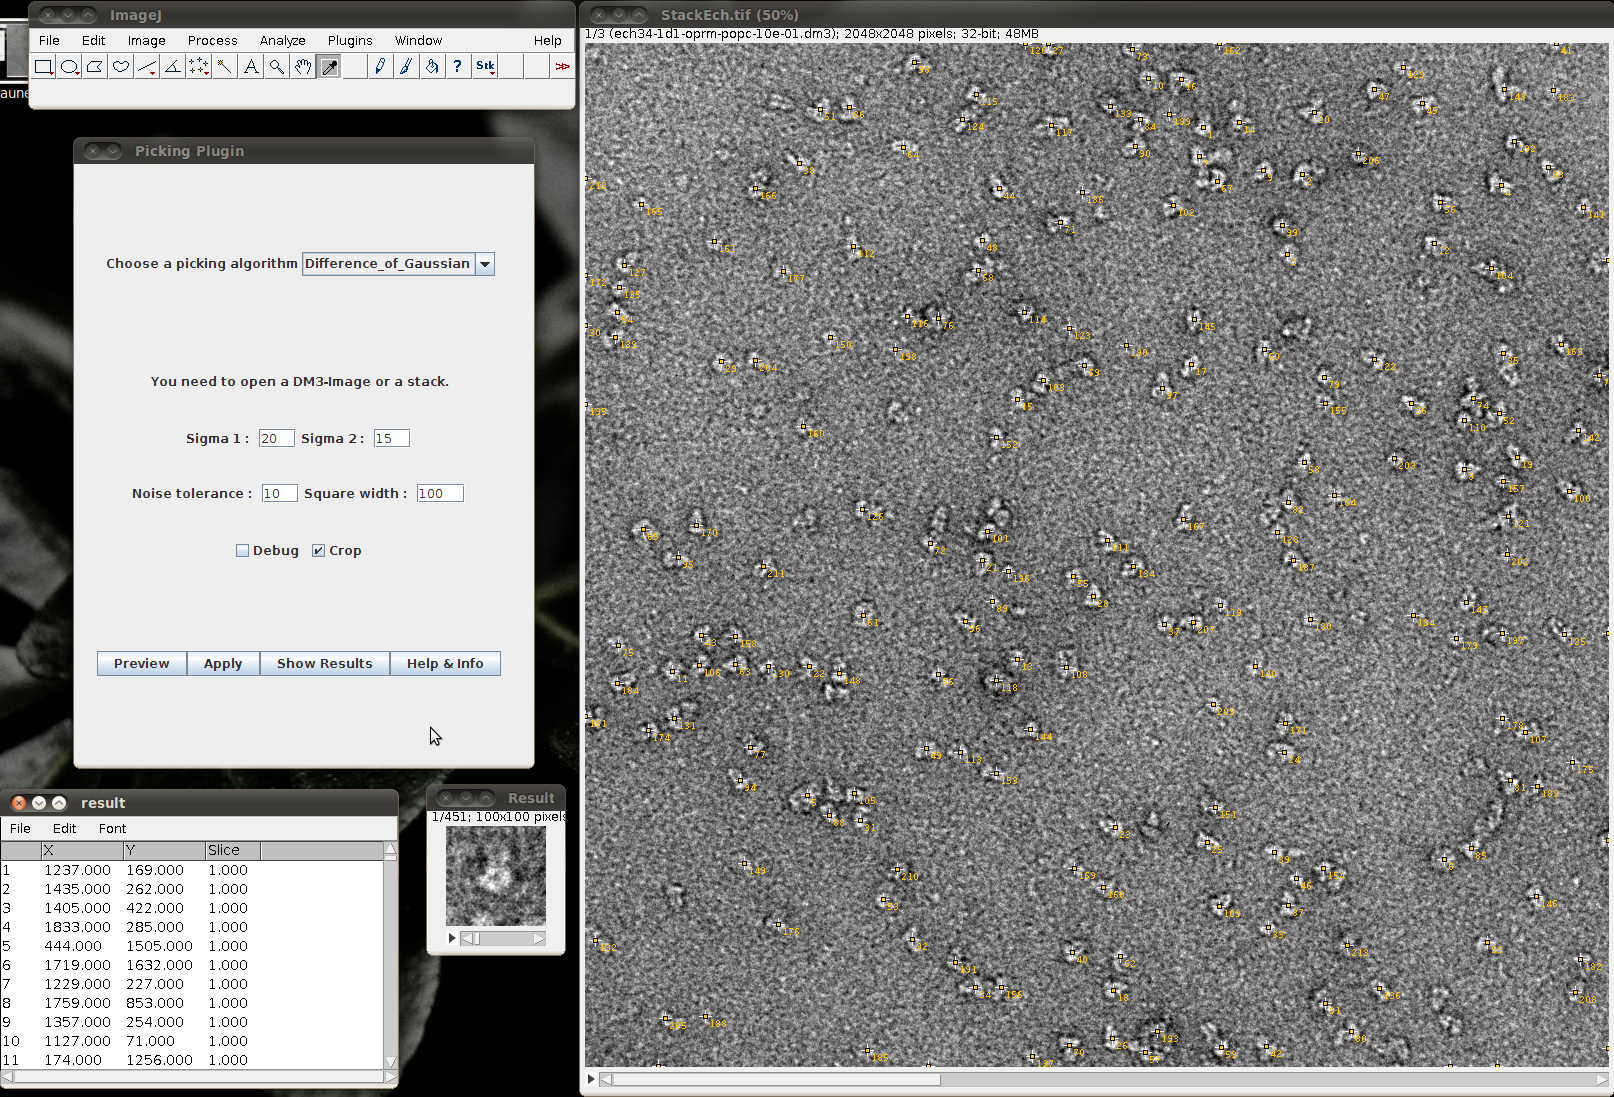
\includegraphics[width=1\textwidth]{Visuel.png}
\caption{Rendu visuel attendu du plugin de picking}
\label{visuel}
\end{center}
\end{figure}

\section{\'Etat de l'existant}

\subsection{Détection à l'aide de références}

Cette technique est utilisée pour trouver des particules dans une image en la comparant à un modèle. Celui-ci peut \^etre obtenu soit à partir d'une structure tridimensionnelle connue, soit par sélection d'une particule servant d'exemple dans les micrographies. L'algorithme détermine la meilleure correspondance entre la cible et le modèle pour pouvoir le localiser dans l'image.%

\subsection{Piquage de particules sans référence}

\subsubsection{Détection des bords et transformée de Hough}

%$\textcolor{red}{(ref:Automatic Particle Detection Through Efficient Hough Transforms
%by Yuanxin Zhu, Bridget Carragher, Fabrice Mouche, and Clinton S.Potter
%IEEE TRANSACTIONS ON MEDICAL IMAGING,VOL.22,N0.9,September 2003)}$\\


%$\textcolor{red}{(ref:http://en.wikipedia.org/wiki/Hough_transform)}$\\
\paragraph*{}
Les difficultés majeures rencontrées dans les techniques basées sur la détection des contours sont dues à la complexité de détecter les bords des particules lorsqu'il y a un bruit de fond important sur les images de MET.%

\noindent
Cette technique est basée sur la détection des contours ainsi que sur l'application de la transformée de Hough~\cite{PdetectEHT:article}. Cette méthode permet de détecter la présence de formes comme des lignes, des cercles ou encore des ellipses.%

\noindent
Dans la transformée de Hough\cite{HT:url} appliquée à la détection de lignes, pour chaque pixel allumé de l'image on trace toutes les lignes possibles, on obtient alors une sinusoïde unique appelée espace de Hough. Si les courbes associées à deux points se coupent, l'endroit où elles se coupent dans l'espace de Hough correspond aux paramètres d'une droite qui relie ces deux points (ordonnée à l'origine et pente).%

\paragraph*{}
La détection de formes qui nous intéressent s’apparentant à des cercles ou des axes circulaires se fait en détectant le centre de celles-ci.
Pour chaque pixel allumé, la fonction trace un cercle de rayon donné. Si la forme a le même rayon que le cercle tracé, tous les cercles se recoupent au centre de la forme, on constate ainsi une amplification de la valeur du pixel central.

\paragraph*{}
D'autre part, pour détecter des particules de formes irrégulières, l'approche décrite précédemment peut également \^etre utilisée mais la transformée de Hough devra alors \^etre remplacée par la transformée de Hough Généralisée~\cite{GHT:url}.
Cette nouvelle méthode repose sur la modification de la transformée de Hough en utilisant le principe de l'identification à partir d'un modèle de référence.
%$\textcolor{red}{(ref:http://en.wikipedia.org/wiki/Generalised_Hough_transform)}$\\

\subsubsection{DoGLFC et classement par affinité}

%$\textcolor{red}{(ref: Reference-free particle selection enhanced with semi-supervised machine learning for cryo-electron microscopy
%by Robert Langlois, Jesper Pallesen, Joachim Frank
%Journal of Structural Biology 175, (2011)353-361)}$
\paragraph*{}
Cette technique est basée sur l'utilisation de l'algorithme DoGLFC\footnote{Difference Of Gaussian Local Fast Correlation} complété par l'algorithme de classement par affinité~\cite{DoGAff:article}.

\paragraph*{}
Le DoGLFC est basé sur l'algorithme DoG Picker du Scripps Institute\cite{Scripps:url}, une méthode rapide qui permet la segmentation de particules. Après l'application de l'algorithme de Différence de Gaussiennes (DoG), on obtient une cartographie de points similaire à celle de la méthode utilisant un modèle de référence.%\blue {\Large ?!} \black %

\noindent
Cet algorithme requiert un paramètre ajustable unique ou un jeu de paramètres basé sur le rayon de la particule ou un ordre de grandeur du rayon. L'exécution de cet algorithme renvoie une liste de trois paramètres décrivant la localisation de la particule (les coordonnées \emph{x} et \emph{y}) et la hauteur du pic.%

\noindent
L'algorithme DoGLFC sélectionne les particules (ou objets) potentielles de taille déterminée, ceci a un pouvoir discriminatif moindre par rapport à une technique basée sur un modèle de référence.

\paragraph*{}
Pour améliorer le rendement lors du piquage des particules, un nouvel algorithme semi-supervisé, le classement par affinité, peut \^etre appliqué.

\noindent
L’algorithme a besoin de trois paramètres d'entrée: un jeu d'images, la taille minimale de l'image après réduction et deux références indiquant quelle fen\^etre doit \^etre utilisée comme référence positive ou négative.

\noindent
Lorsque l'algorithme a fini de se dérouler, on obtient une classement pour chaque fen\^etre où le maximum correspond à la particule ciblée.

\paragraph*{}
L'utilisation de DoGLFC complété par le classement par affinité permet d'extraire
rapidement les particules de l'image et d'éliminer avec précision les particules correspondant à de la contamination ou du bruit de fond.

\subsection{Perceptron}

\paragraph*{}
Un perceptron est une sorte de réseau neuronal artificiel. Dans son état le plus simple, il représente un système de classification binaire/linéaire.%

\noindent
Ce programme a la particularité d'être capable d'apprendre des concepts, ce qui signifie qu'il peut apprendre afin de répondre par vrai ou faux à des données qui lui sont soumises, gr\^ace à la présentation répétée de plusieurs exemples d'étude.
Il a déjà été testé sur des images binaires pour la détection de formes ou de contours mais pas sur des images en niveaux de gris ou sur des problèmes de reconnaissance de modèles visant à sélectionner des particules. Le réseau neuronal n'a pas non plus été exploité comme un outil de sélection automatique de particules mais plusieurs recherches ont conclu qu'il pourrait \^etre utilisé pour l'élimination de faux-positifs.~\cite{Perceptron:article}.%

\section{Analyse des besoins}

\noindent
Ils sont de deux types: fonctionnels et non fonctionnels, et diffèrent entre l'interface utilisateur et les algorithmes de piquage.

\subsection{Besoins fonctionnels}

\subsubsection{Interface}

\noindent
Au lancement, les images sont préalablement chargées sur \imj , l'utilisateur a le choix entre plusieurs algorithmes de piquage. %L'interface propose un mode de prévisualisation afin de vérifier le piquage sur une image avant de l'appliquer au stack entier.
Nous avons essayé de faire en sorte que l'affichage soit clair et succinct, constitué d'un menu déroulant, d'une liste de boutons et d'une interface propre à chaque algorithme.\\
Enfin, il est également possible d'implanter simplement de nouveaux algorithmes dans l'interface. % Simplement, ou pas ^^

\subsubsection{Les algorithmes}

Les algorithmes implantés doivent réaliser un piquage automatique des particules depuis les micrographies issues de \me. Le format de sortie est un tableau de résultats contenant un jeu de coordonnées \emph{x, y} associé à la position de l'image dans la pile d'images (\textit{stack} en anglais), ainsi qu'une nouvelle pile contenant les particules sélectionnées par l'algorithme si l'utilisateur le désire.

\subsection{Besoins non fonctionnels}

\subsubsection{Interface}

\noindent
L'implémentation de la plateforme a été réalisée en \java, nous utilisons les API\footnote{Application Programming Interface} graphiques de la bibliothèque \emph{Swing}. 
Il s'agit d'une interface graphique (GUI)\footnote{Graphic User Interface} faisant partie du paquetage Java Foundation Classes (JFC), inclus dans J2SE. Cela constitue une des principales évolutions apportées par Java2 par rapport aux versions antérieures. Elle offre la possibilité de créer des interfaces graphiques identiques quelque soit de système d'exploitation sous-jacent, au prix de performances moindres qu'en utilisant Abstract Window Toolkit (AWT) l'autre bibliothèque principale pour \java. \\
De plus, nous avons essayé de faire en sorte que le programme soit le plus simple d'utilisation possible afin de le rendre accessible à tous. C'est pourquoi nous avons tenté de faire un code clair, explicite et commenté afin de permettre aisément l'implémentation de nouveaux algorithmes.

\subsubsection{Les algorithmes}

\noindent
Les algorithmes ont été testés avec l'outil macro d' \imj ~puis implémentés en \java. Nous avons fait en sorte que le temps de déroulement de l'algorithme soit assez rapide afin de pouvoir gérer de grands jeux de données et qu'aucune image de traitement intermédiaire n'apparaisse à l'utilisateur (à moins qu'il ne le souhaite).\\

Dans l'optique de démocratiser l'utilisation de notre interface et afin de permettre l'extension de ce plugin avec d'autres algorithmes, le projet a été placé sous une licence GPL\footnote{General Public License~\cite{GPL:url}}.

\noindent
%Le projet devra être terminé vers mi-mai. %prière de nous mettre une bonne note !

\section{Scénario d'utilisation du plugin}

Nous prendrons l'exemple d'une image issue de \cme ~collectée dans l'équipe ACMPC sur laquelle se trouvent des protéines membranaires que nous voulons sélectionner (Figure \ref{prot}) ainsi que d'une image utilisée comme référence sur \imj ~, les \emph{blobs} (Figure \ref{blobs1}).

\begin{figure}[!ht]
\begin{center}
 \begin{minipage}{.450\linewidth}
  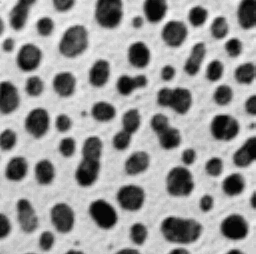
\includegraphics[width=0.92\textwidth]{blobs.png}  
  \caption{Image Blobs de réference}
  \label{blobs1}
 \end{minipage} \hfill
\begin{minipage}{.450\linewidth}
  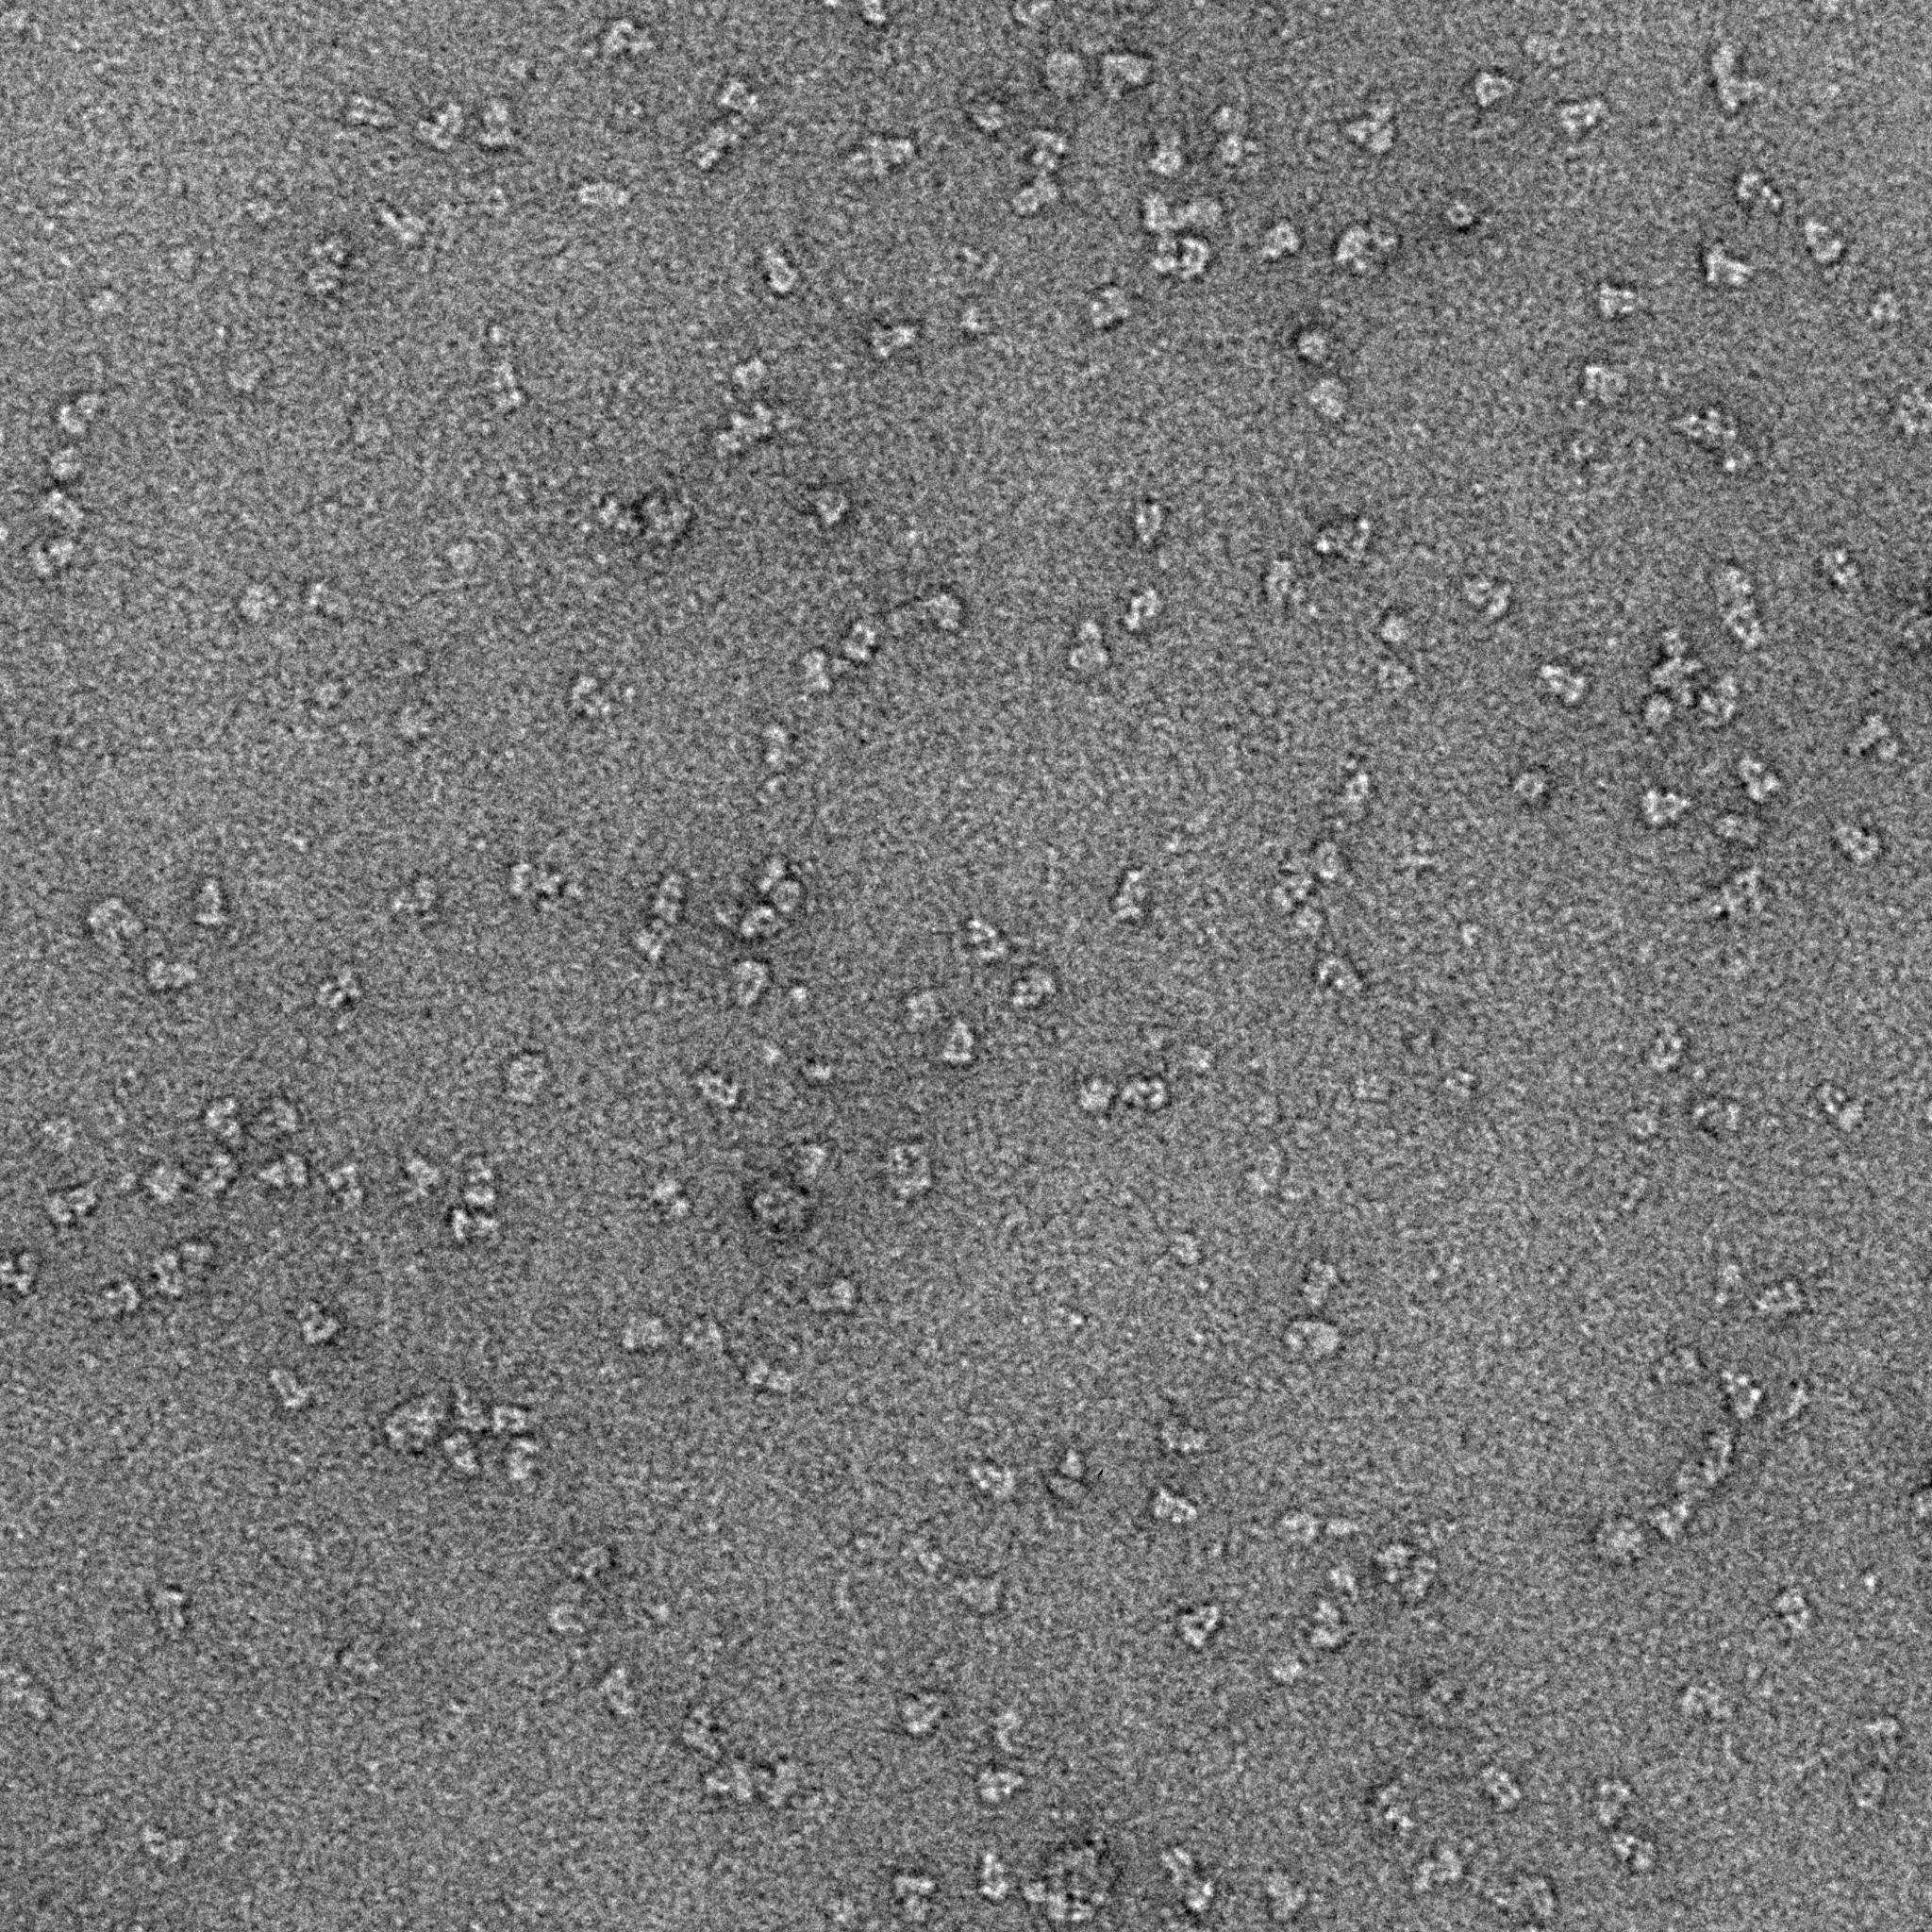
\includegraphics[width=0.98\textwidth]{proteines.jpg}   
  \caption{Image de protéines membranaires observées au \me}
  \label{prot}
 \end{minipage} \hfill
%\caption{Exemple d'images formant le stack de particules (blobs et protéines)}
\end{center}
\end{figure}

%\begin{figure}[h] 
%\begin{center}
%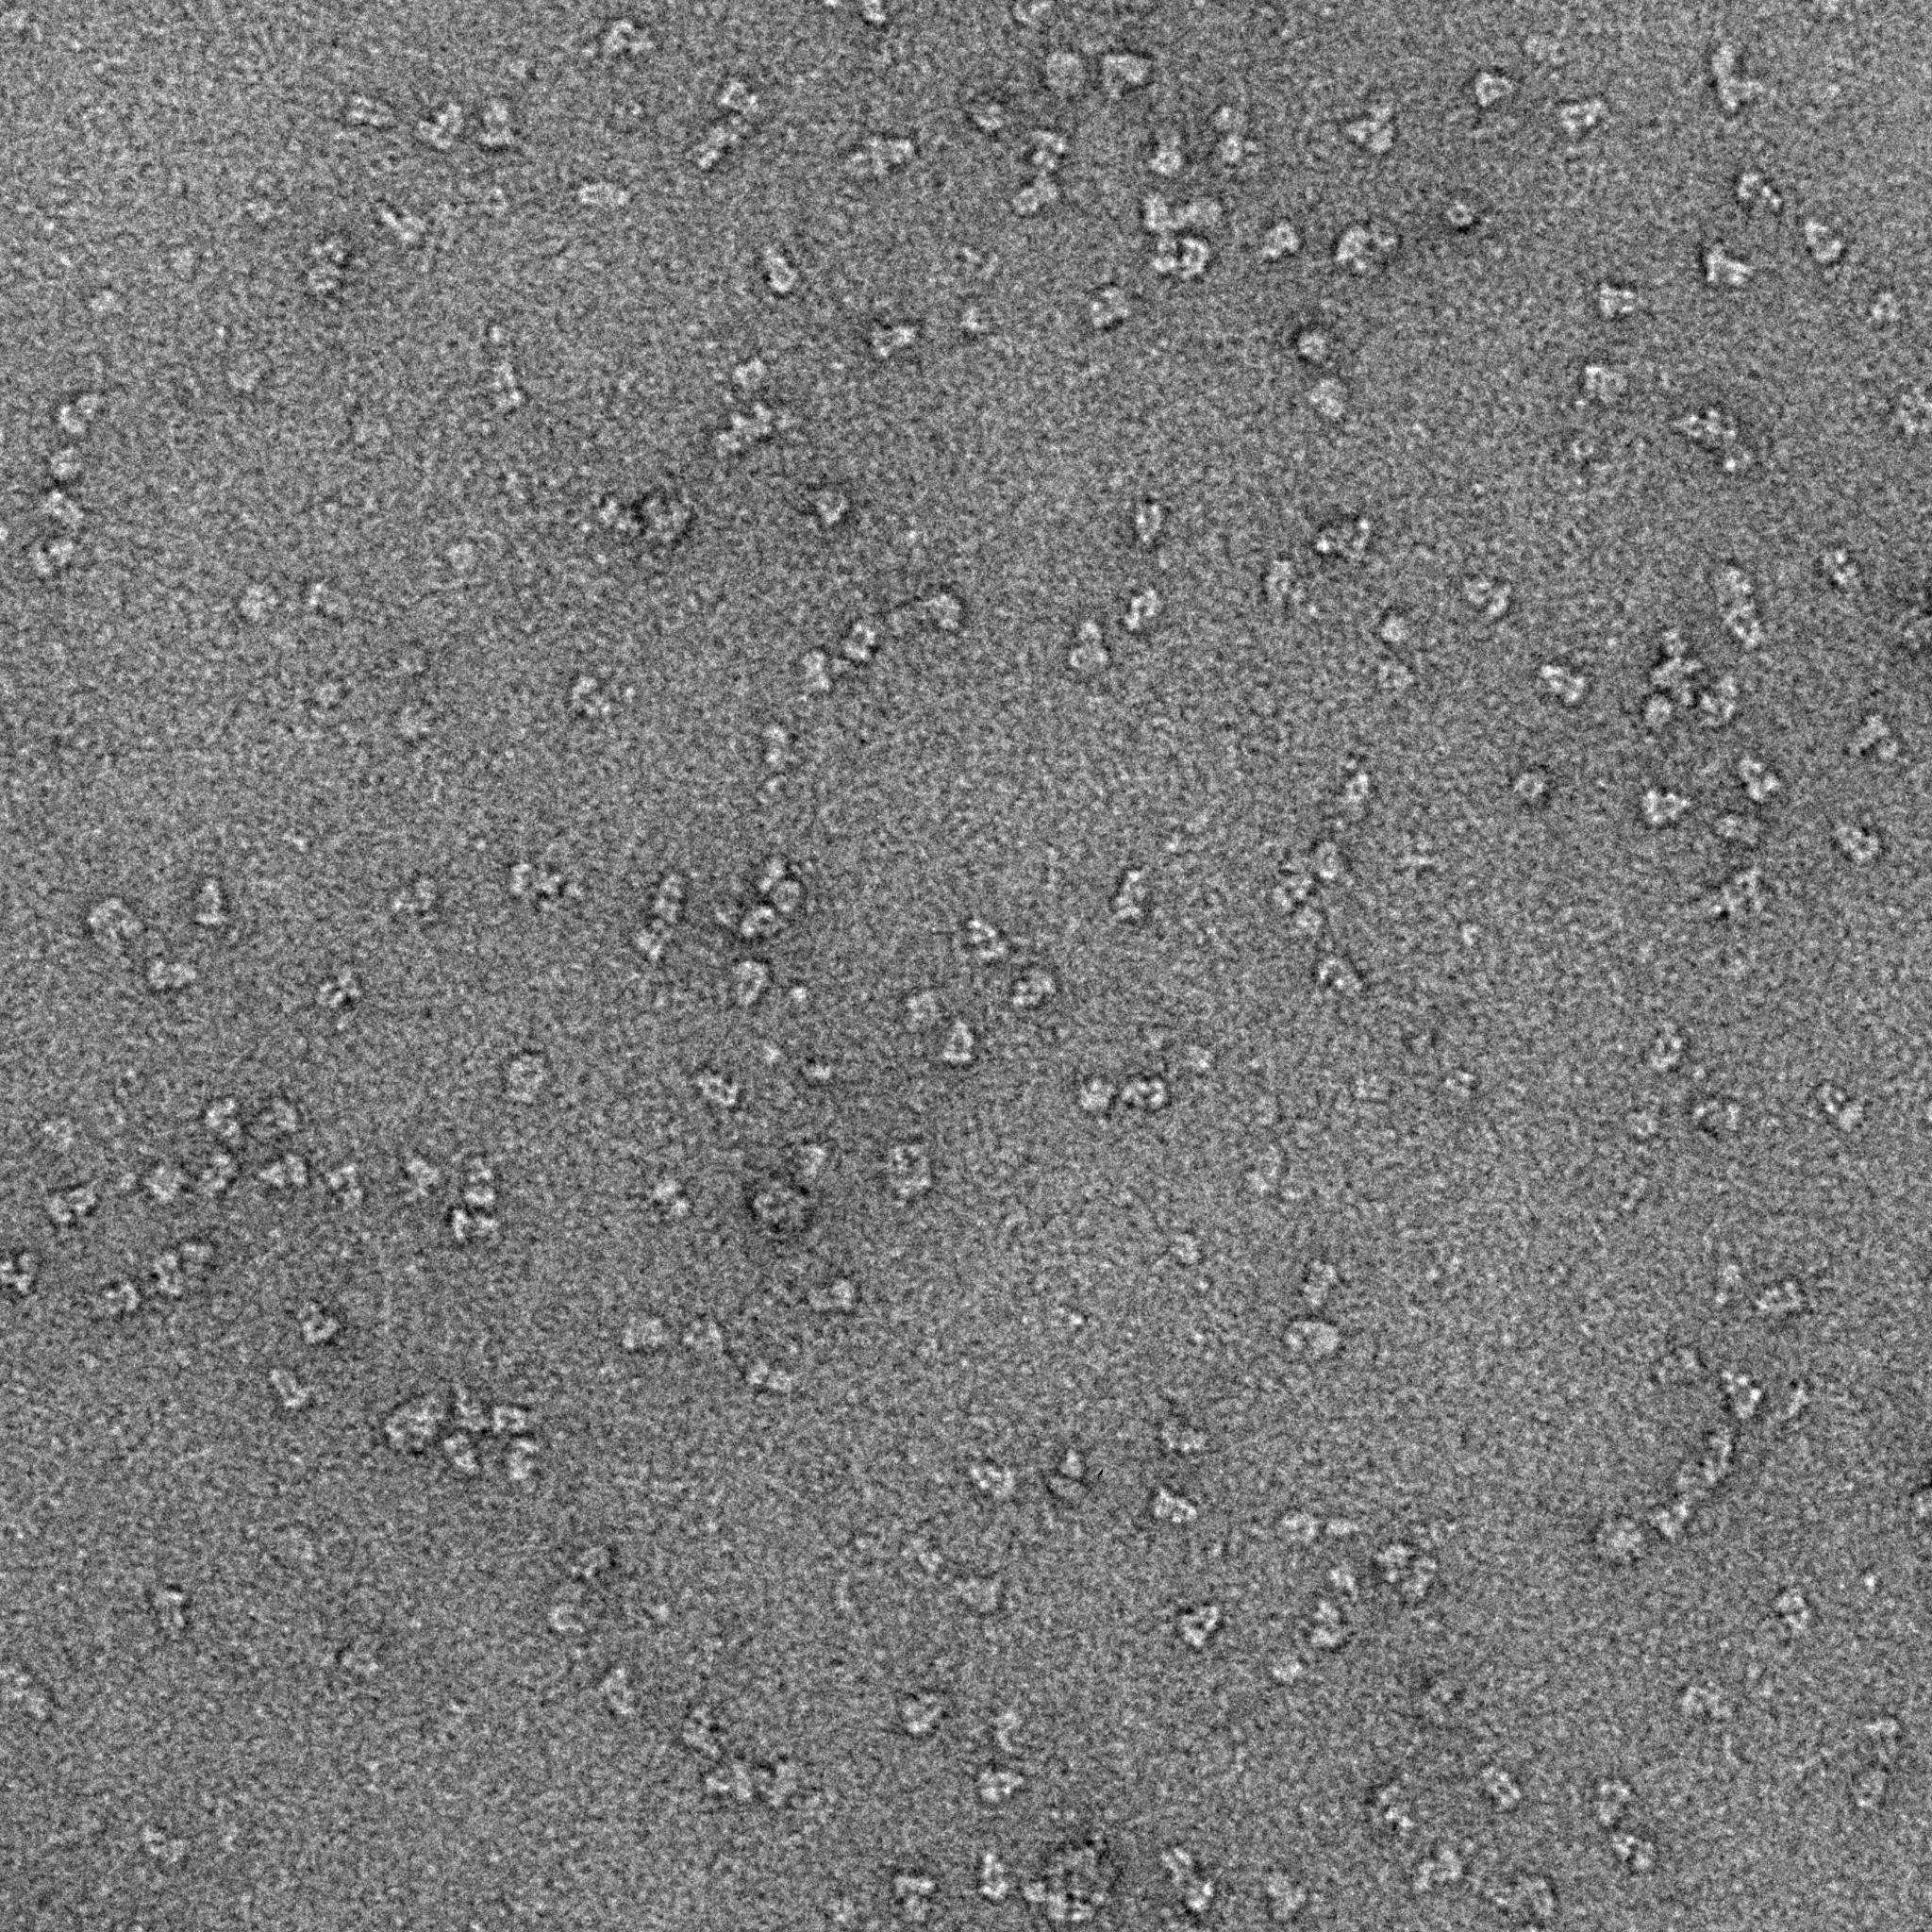
\includegraphics[width=0.5\textwidth]{proteines.jpg}
%\caption{Image de protéines membranaires observées au \me}
%\label{prot}
%\end{center}
%\end{figure}

Nous avons tenté de nous mettre à la place d'un chercheur pour avoir une vision biologique de l'utilisation de notre plugin. Tout au long de ce rapport, vous pourrez donc suivre toutes les procédures qui nous ont permis de réaliser la sélection. 



\newcommand{\black}{\color{black}}
\newcommand{\blue}{\color{blue}}

\chapter{Conception}

\section{Interface graphique}

Comme précisé précédemment, notre programme se présente sous la forme d'un plugin \imj . L'interface graphique a été réalisée grâce à la bibliothèque  \java ~Swing. 
La fenêtre servant d'interface est composée de différentes boîtes (panneaux) contenant différents outils (boutons, listes, zones de saisie et zones de texte) permettant l'interaction entre l'utilisateur et le programme. Ces boîtes peuvent s'imbriquer les unes dans les autres afin d'obtenir des structures plus complexes et un meilleur rendu visuel. \\
L'interface du plugin est simple, elle prend la forme d'une fenêtre composée d'un menu déroulant, dans lequel se trouvent les différents algorithmes, et de quatre boutons. 

\subsection{Panneaux}

La Figure \ref{panneaux} donne un aperçu de l'organisation des différents panneaux de notre interface. Celle-ci est composée d'une arborescence de panneaux comportant un panneau principal (en bleu, permettant d'organiser la fenêtre du plugin), lui-m\^eme constitué des trois panneaux subsidiaires (en orange) suivants :
\begin{description}
\item \textbf{Le premier panneau} contient une liste déroulante permettant le choix de l'algorithme. 
\item \textbf{Le panneau du milieu} est vide au lancement du plugin et s'actualise en fonction de l'algorithme de piquage choisi. Il affiche une aide rapide sur les conditions d'utilisation de l'algorithme de piquage, les zones de saisies utilisateur propre à cet algorithme. Il affiche également les choix génériques : mode de débogage, mode de découpe des sélections et taille de la sélection, gestion du bruit de fond. \\
Tout cela s'organise à l'aide de sous-panneaux (en violet).
\item \textbf{Le dernier panneau} contient les boutons d'actions : prévisualisation, exécution, affichage des résultats, informations/aide.
\item \textbf{Le panneau principal} permet notamment d'imposer la taille de l'interface.
\end{description}

\begin{figure}[!h] 
\begin{center}
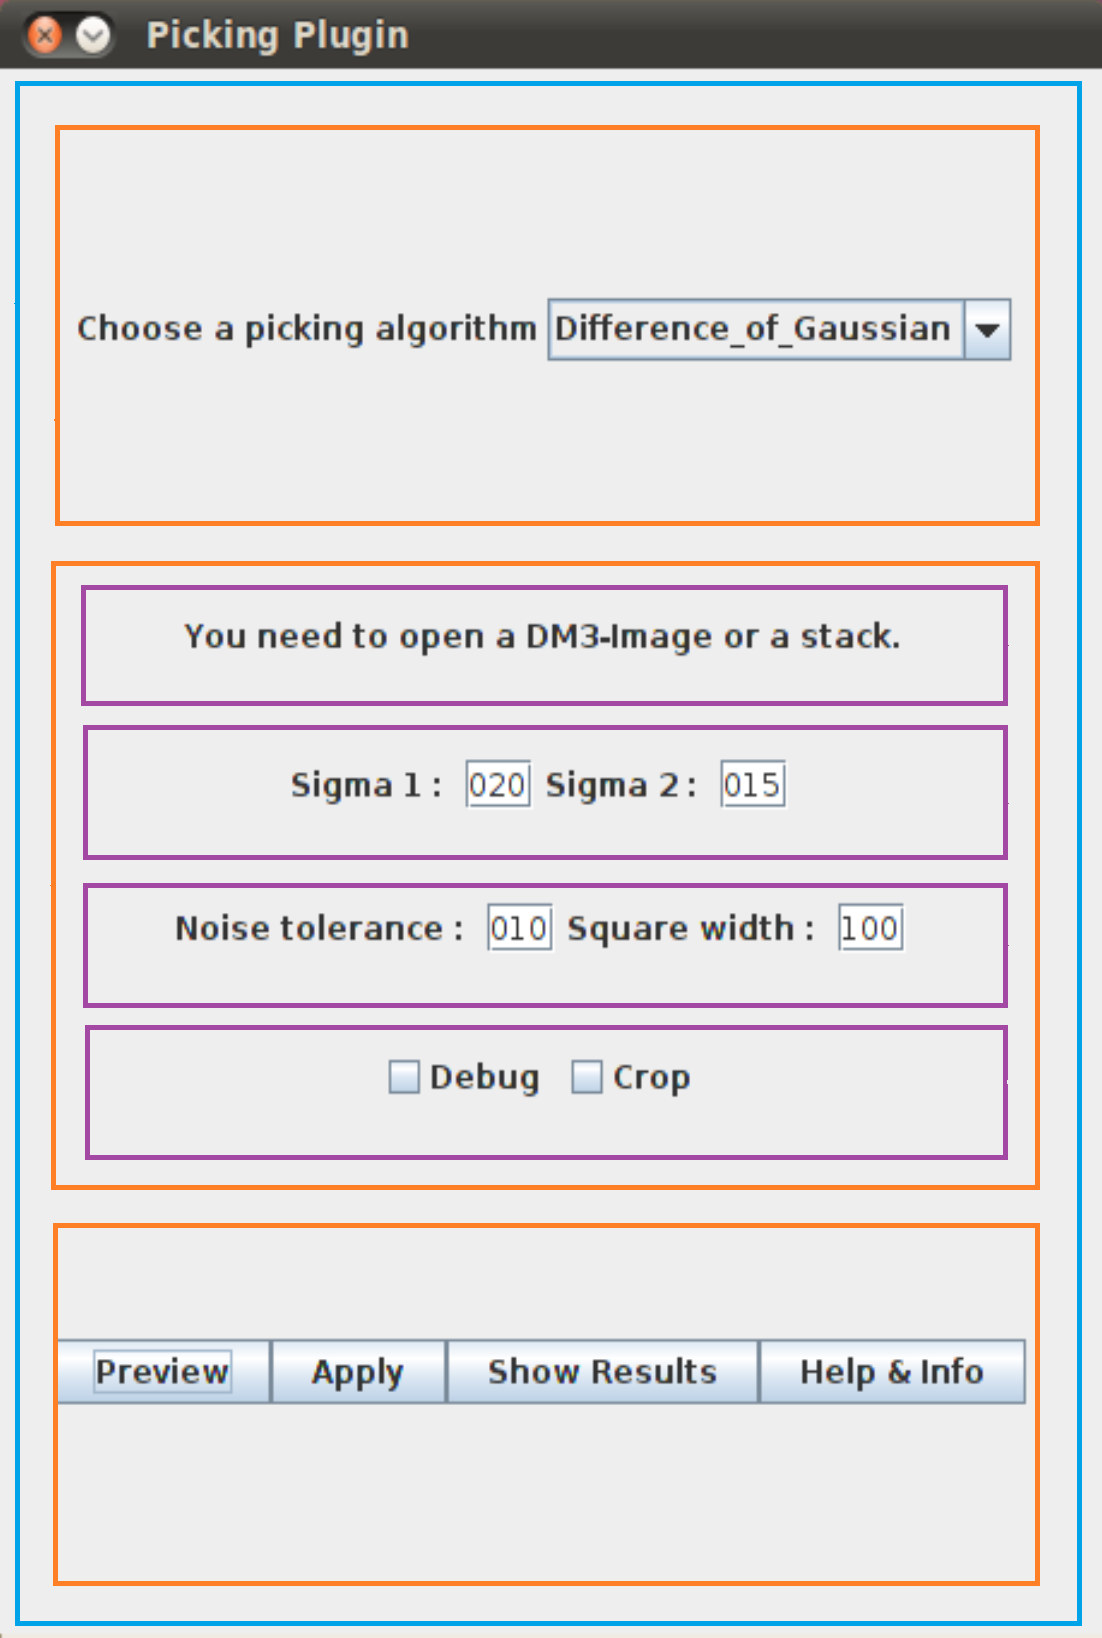
\includegraphics[width=0.4\textwidth]{pluginCadres.png}
\caption{Organisation des panneaux pour l'algorithme Difference of Gaussian}
\label{panneaux}
\end{center}
\end{figure}
\pagebreak

\subsection{Boutons}

Les boutons doivent répondre aux clics de la souris et lancer l'action correspondante en fonction de l'algorithme de piquage choisi par l'utilisateur :

\begin{description}
\item \textbf{Le bouton de prévisualisation} permet de tester le piquage obtenu par l'algorithme sélectionné sur l'image courante.
\item \textbf{Le bouton d'exécution} permet d'appliquer l'algorithme sur l'image ou la pile d'images sélectionnée, lorsque l'utilisateur est s\^ur des paramètres qu'il souhaite appliquer.
\item \textbf{Le bouton d'information/aide} est une aide d'utilisation du plugin ainsi que des conditions de fonctionnement des algorithmes.
\item \textbf{Le bouton d'affichage des résultats} permet d'afficher et de sauvegarder le tableau des coordonnées des particules sélectionnées.% avec l'aide d'\imj.  
\end{description}
Pour que le plugin puisse fonctionner, l'utilisateur devra au préalable avoir ouvert une image ou un \textit{stack} d'images à l'aide d'\imj.
\pagebreak

\section{Récupération des paramètres}

Les méthodes de piquage ont une classe mère commune. L'utilisateur sélectionne un algorithme dans le menu déroulant et détermine certains paramètres. Quelques uns sont propres aux algorithmes et d'autres sont communs à tous tels que :

\begin{itemize}
\item la gestion du bruit de fond,
\item la taille des images des particules sélectionnées lorsqu'on demande le \textit{stack} d'images,
\item l'activation du débogage (s'il est implémenté dans l'algorithme),
\item l'activation du découpage des particules à partir du piquage obtenu.
\end{itemize}

\section{Algorithmes}

\subsection{Corrélation d'image}

La méthode par corrélation croisée donne des résultats similaires à une transformée de Hough pour des objets circulaires. Elle produit une carte de corrélation entre une référence (dans notre cas, un cercle de taille définie) et une image de MET contenant des particules circulaires. Chaque pixel de cette carte correspond à la mesure de similarité entre les deux images. Les valeurs élevées des pixels représentent donc les meilleures similarités et permettent de localiser les particules circulaires de même rayon que celle de l'image de référence. Cette opération est réalisée en espace fréquentiel via une Transformée de Fourier et est déjà implantée dans ImageJ. \\
Par rapport à la transformée de Hough, la corrélation croisée est beaucoup plus rapide mais est réservée (pour l'implantation dans ImageJ) à des images carrées dont le côté doit être une puissance de 2. Cet inconvénient ne nous gêne pas car les images de MET sont de 2048x2048 pixels (et la plupart des traitements sont appliqués à des images réduites de 1024x1024). \\

\noindent
Pour cette méthode de piquage, plusieurs images de référence sont utilisées avec des cercles de divers rayons afin de sélectionner toutes les particules circulaires des images de MET. L'utilisateur doit entrer les rayons minimal et maximal des particules à sélectionner, ainsi que la valeur de l'incrément. \\
Pour un résultat optimal, avant de lancer la sélection des particules avec cet algorithme, l'utilisateur devra traiter l'image pour éliminer un maximum de bruit de fond (utilisation de filtres).

\subsection{Différence de Gaussiennes (DoG pour \textit{Difference of Gaussian})}

La différence de Gaussiennes est une technique qui soustrait une image à laquelle a été appliqué un filtre gaussien à une deuxième image, elle aussi filtrée (par le m\^eme filtre) mais en utilisant une valeur d'écart-type plus petite, donc moins filtrée. Par conséquent, les bords des particules sont dégradés, nous permettant de récupérer les maxima de l'image résultante, c'est-à-dire le centre des particules.\\
%La différence de Gauss est une technique qui consiste en la soustraction d'une version floutée %de l'image d'origine à une autre version moins floutée de cette même image.\\
\noindent
Il est demandé à l'utilisateur d'entrer les valeurs d'écart-type qui seront utilisées pour appliquer les filtres gaussiens.

\subsection{Extraction de contours}

Cette méthode (aussi appelée "Différence de dilatation") repose sur le même principe que la Différence de Gaussiennes, mais en utilisant des opérateurs de morphologie mathématique (érosion et dilatation). Nous lui appliquons un certain nombre de cycles de dilatation et obtenons alors des particules de plus grande taille. A la soustraction des deux images, seuls les contours des particules apparaîtront, nous permettant de récupérer le centre de particules.\\
L'utilisateur devra entrer le nombre de cycles de dilatation qu'il souhaite appliquer à chaque image.

\section{Pile d'images résultantes}

Si l'utilisateur le désire, il peut récupérer une pile d'images contenant les particules piquées. Celle-ci est obtenue à partir du tableau des coordonnées que la fonction de création du \textit{stack} prend en paramètre d'entrée.
Les particules trop près du bord sont éliminées, les autres ajoutées dans un \textit{stack} qui est finalement affiché à l'utilisateur.

\section{Organisation orientée objet du programme}

Afin de clarifier et de simplifier le code, nous avons tenté de séparer les grandes fonctions du programme en suivant les principes de la programmation orientée objet.

\subsection{Séparation interface graphique et traitement d'images}

Sans suivre le patron de conception Modèle-Vue-Controleur (MVC~\cite{mvc:url}), nous avons créé différentes classes permettant de distinguer la partie GUI de la partie algorithme. Nous obtenons ainsi des classes ne gérant que l'aspect graphique du plugin. Celles-ci gèrent plus particulièrement les panneaux propres aux méthodes de piquage ainsi que les classes bien distinctes effectuant les traitements d'images.

\subsection{Séparation traitement d'images et création du \textit{stack}}

La partie permettant la création du \textit{stack} d'images individuelles a été séparée des méthodes de piquage afin d'éviter la répétition de ce code dans chaque algorithme. Cela permet aussi d'y faire appel en dehors de nos algorithmes, contrairement à une implémentation de cette fonction dans une classe mère.

\subsection{Patrons de conception}

Cette séparation GUI/traitement/\textit{stack} à dû être accompagnée de la création de classes suivant des patrons de conception particulier : la \emph{factory} et le \emph{singleton}. 
\begin{description}
\item [Le \emph{singleton}] est un patron de conception (\textit{design pattern}) permettant de restreindre l'instanciation d'une classe à un seul objet (ou bien à quelques objets seulement). La classe \texttt{Attributes} en \emph{singleton} permet de conserver les paramètres choisis par l'utilisateur. De ce fait, même lorsqu'il exécute plusieurs algorithmes, une seule instance de cette classe peut exister, actualisant les paramètres choisis par l'utilisateur.
\item[La \emph{factory}] définit une interface pour la création d'objets (ou groupes d'objets). La classe \texttt{AlgoFactory} en \emph{factory} rend possible les transitions entre chaque méthode de piquage. Elle amorce le panneau propre à l'algorithme permettant d'actualiser l'interface et ainsi de récupérer les paramètres utilisateur. Ensuite, lorsque l'utilisateur clique sur les boutons d'exécution ou de prévisualisation, la \emph{factory} lancera les actions correspondantes. Afin d'éviter des erreurs d'instanciations, cette classe suit également le patron de conception \emph{singleton}.
%\item [Le \emph{singleton}] est un patron de conception (design pattern) permettant de restreindre l'instanciation d'une classe à un seul objet (ou bien à quelques objets seulement). La classe en \emph{singleton} permet de conserver les paramètres choisis par l'utilisateur. De ce fait, même lorsqu'il exécute plusieurs algorithmes, une seule instance de cette classe peut exister, actualisant les paramètres choisis par l'utilisateur.
\end{description}

\subsection{Modularité et réutilisation du code}

L'organisation orientée objet du programme a fortement facilité l'écriture du programme, évitant la répétition de lignes de code qui pouvaient \^etre factorisées. De plus, cela permet une grande modularité au sein de notre programme, facilitant l'ajout ou le retrait d'un algorithme de piquage et de son interface dans notre plugin. Cette modularité est telle qu'elle permet, en ce qui concerne le module de création du \textit{stack} de particules sélectionnées, de l'utiliser en dehors de notre plugin.\\
Cela tient un rôle important dans notre projet car, comme pour beaucoup de logiciels libres, \imj ~se développe énormément gr\^ace à sa communauté d'utilisateurs qui participe au développement de plugins. Après validation par le personnel du NIH \footnote{National Institute of Health} responsable de ce projet, les plugins sont mis à la disposition des utilisateurs. Ainsi, chacun pourrait ajouter/améliorer des méthodes de piquage de particules, développant et augmentant l'efficacité et la sélectivité de notre plugin. \\

Ci-après (Figure \ref{classes}) le diagramme général de l'organisation de nos classes :

\begin{figure}[!h] 
\begin{center}
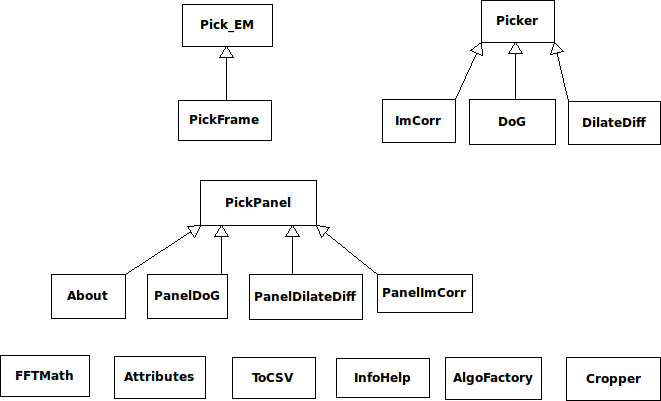
\includegraphics[width=0.8\textwidth]{class_diagram.png}
\caption{Organisation générale des classes du plugin Pick\_EM}
\label{classes}
\end{center}
\end{figure}

\pagebreak
Afin de faciliter la portabilité de notre plugin, nous avons choisi de le compresser au format \emph{JAR\footnote{Java ARchive\cite{jar:url}}} qui est un fichier ZIP\footnote{Format de fichier permettant l'archivage et la compression de données sans perte de qualité \cite{zip:url}} utilisé pour distribuer un ensemble de classes \java. Ce format est utilisé pour stocker les définitions des classes, constituant l'ensemble d'un programme.
Ce format est directement pris en compte par \imj ~et, lorsque l'archive est placée dans le dossier correspondant, directement ajouté au menu des plugins.\\

Cette archive contient les fichiers source \emph{.java} pour permettre la modification du code et les fichiers compilés \emph{.class} afin de permettre l'utilisation du plugin sans avoir de problèmes de compilation (généralement dus à la version de \java ). \\

Du fait que notre plugin soit \textit{open-source} et en libre accès, il était important de protéger l'accès à notre travail. Pour cela, nous avons décidé de placer notre programme sous licence. \\
Plusieurs types de licence étaient envisageables, notamment les licences \emph{GPL}, L-\emph{GPL}, \emph{BSD} pour celles en anglais, et les licences \emph{CéCill} pour celles propres à la législation française. Sur l'avis de nos tuteurs, mais aussi parce que c'est celle la plus couramment utilisée pour les plugins \imj , nous avons choisi la licence \emph{GPL} qui est la plus permissive tout en nous garantissant l'accès à notre travail. 



\newsavebox{\fmbox}
\newenvironment{fmpage}[1]
     {\begin{lrbox}{\fmbox}\begin{minipage}{#1}}
     {\end{minipage}\end{lrbox}\fbox{\usebox{\fmbox}}}

\chapter{Réalisation}

Sous \imj, il existe deux types de plugins : \emph{PlugInFilter} et \emph{PlugInFrame}. Étant donné que nous avions besoin de différents objets graphiques, nous avons choisi d'utiliser \emph{PlugInFrame}. C'est la classe \texttt{Pick\_EM} qui en hérite et permet de lancer notre plugin à son appel par l'intermédiaire de la barre de menus d'\imj.

\section{Interface graphique}

\subsection{Panneaux et boutons}

Nos panneaux dérivent de la classe \emph{JPanel}, elle-même issue de la classe \emph{Panel}. Cette dernière fournit un composant \emph{Container} permettant d'accueillir d'autres composants graphiques (sous-panneaux).\\

Le premier panneau (\textbf{panel1}) contient une zone de texte (\emph{JLabel}) afin d'afficher un message d'aide, ainsi qu'un menu déroulant (\emph{JComboBox}) pour le choix des algorithmes. \\

Le panneau central (\textbf{panel2}) est vide au lancement du plugin et son contenu varie en fonction de l'algorithme sélectionné. Par exemple pour l'algorithme Difference of Gaussian, les sous-panneaux sont créés dans la classe \texttt{panelDoG}. Pour cet algorithme, le \textbf{panel2} comprend :
\begin{itemize}
\item \textbf{infoPanel} contenant un \emph{JLabel} indiquant le type d'image requis.
\item \textbf{sigmaPanel} et \textbf{widthNoisePanel} qui contiennent des \emph{JLabel} et \emph{JTextField} afin de créer une zone dans laquelle il est possible d'entrer les paramètres nécessaires au déroulement du piquage. 
\item \textbf{debugCropPanel}, quant à lui, contient deux cases à cocher (\emph{JCheckBox}) pour activer ou non les modes de débogage et de crop. 
\end{itemize}
Les classes \texttt{panelImCorr} et \texttt{panelDilateDiff} servent à la création des sous panneaux des algorithmes Image Correlation et Dilate Difference respectivement. \\

Le dernier panneau (\textbf{panel3}) comporte quatre boutons (\emph{JButton}) devant répondre aux clics de la souris à l'aide d'un \emph{ActionListener}. \\

Enfin, le panneau principal (\textbf{mainPanel}) contient tous les panneaux cités précédemment. Sa taille détermine celle de la fenêtre du plugin. \\
Ces quatre panneaux sont crées dans la classe \texttt{PickFrame}, qui hérite de la classe \texttt{JFrame}. \texttt{PickFrame} peut également accéder à des méthodes de la classe \texttt{ActionListener}. \\

\pagebreak
La figure suivante (Figure \ref{panneauxDetail}) donne un aperçu plus visuel de l'organisation de ces différents panneaux.
\begin{figure}[!ht] 
\begin{center}
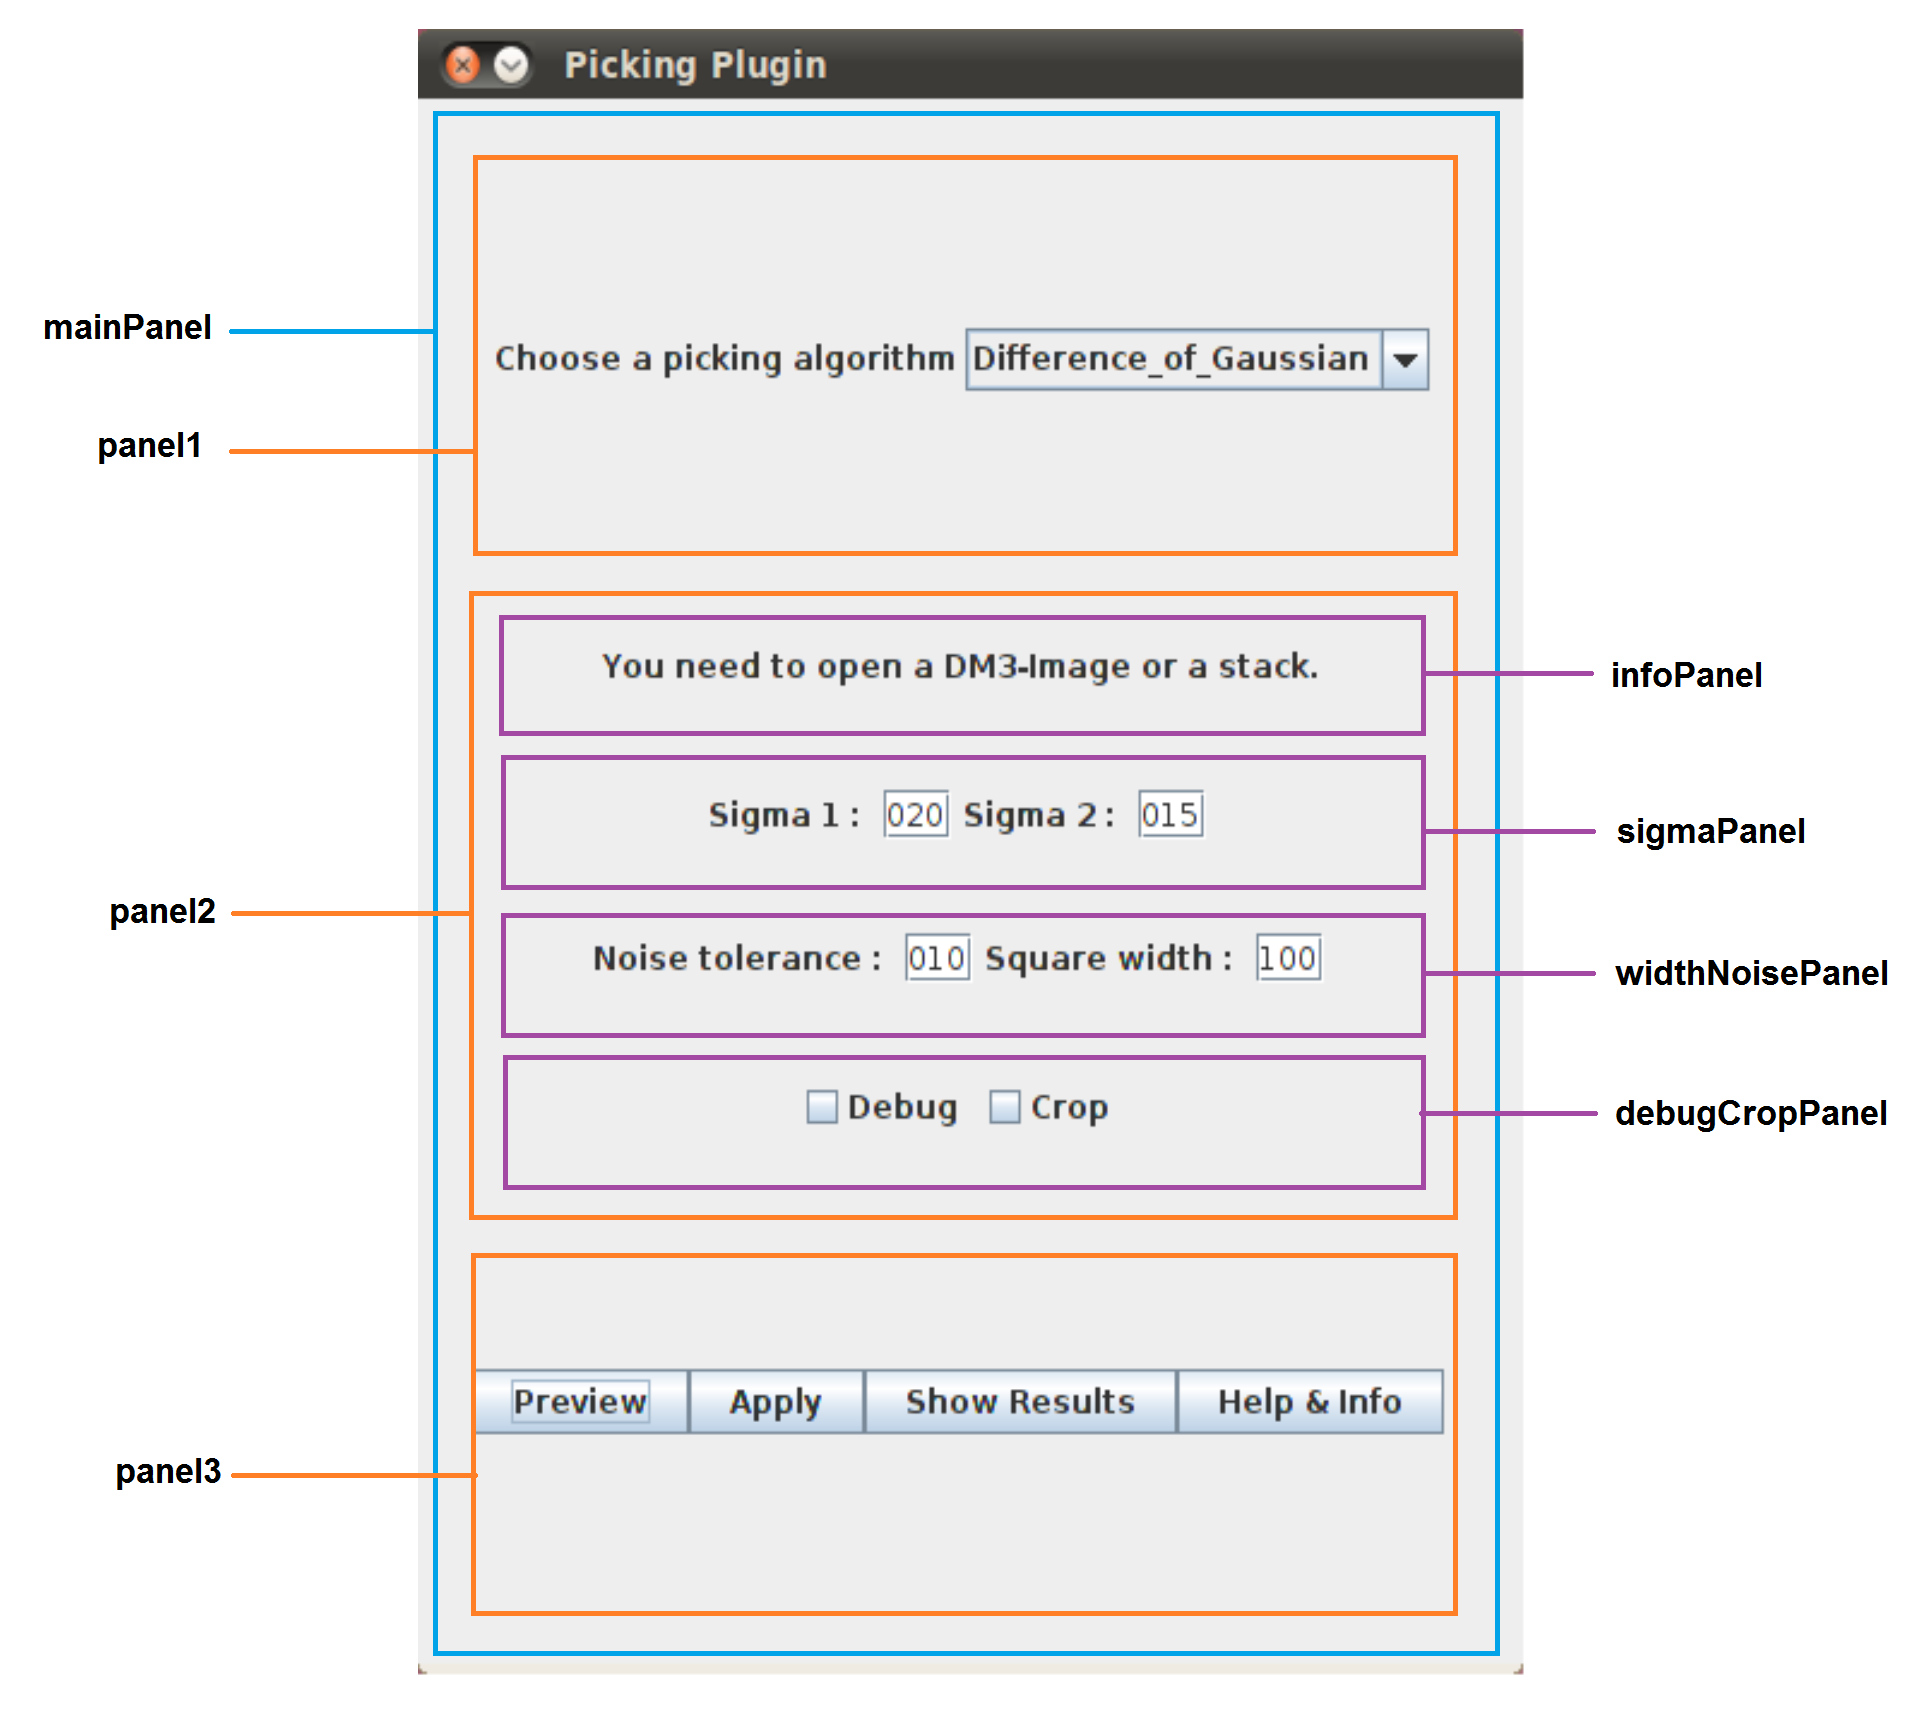
\includegraphics[width=0.8\textwidth]{plugin3-1.png}
\caption{Organisation des panels pour l'algorithme Difference of Gaussian}
\label{panneauxDetail}
\end{center}
\end{figure}

La classe \texttt{PickFrame} permet donc de générer l'interface graphique du plugin. De plus, elle permet de réagir lors d'un clic sur un bouton. C'est la méthode \texttt{actionPerformed()} qui vérifie le nom de l'algorithme choisi par l'utilisateur parmi ceux proposés dans la JComboBox et permet d'afficher le panel2 qu'il faut. Ci-après un extrait de la méthode \texttt{actionPerformed()} :

\begin{center}
\begin{fmpage}{15cm}
\begin{small}
\begin{lstlisting}[breaklines=true, breakatwhitespace=true]
public void actionPerformed(ActionEvent e) {
  String command = e.getActionCommand();
  String comboSelection = null;
  if (command.equals("comboBoxChanged")){
    JComboBox cb = (JComboBox)e.getSource();
    comboSelection = (String) cb.getSelectedItem();
    panel2.removeAll();
    // Allows the panel2's update
    mainPanel.remove(panel1);
    mainPanel.remove(panel2);
    mainPanel.remove(panel3);
    panel2 = AlgoFactory.algorithm.getPickPanel(comboSelection);
    mainPanel.add(panel1);
    mainPanel.add(panel2);
    mainPanel.add(panel3);
    mainPanel.repaint();
    pack();
  }
\end{lstlisting}
\end{small}
\end{fmpage}
\end{center}

\paragraph*{}
Comme nous avions quelques soucis d'actualisation des panneaux, lors de l'implémentation, nous avons décidé de les supprimer puis de les recréer lors de chaque changement d'algorithme. Le chargement du bon panel2 se fait gr\^ace à \texttt{getPickPanel} de la classe \texttt{AlgoFactory}. La méthode \texttt{pack()} permet de recadrer la fenêtre en fonction de son contenu. 

\begin{center}
\begin{fmpage}{15cm}
\begin{small}
\begin{lstlisting}
if (command.equals("Apply")){
  comboSelection = (String)algoList.getSelectedItem();
  Attributes.getInstance();
  coordXYZ = AlgoFactory.algorithm.getPicker(comboSelection);
  IJ.showStatus("End of picking");
}
else if (command.equals("Preview")){
  comboSelection = (String)algoList.getSelectedItem();
  Attributes.getInstance();
  AlgoFactory.algorithm.getPickerPreview(comboSelection);
  IJ.showStatus("End of Preview");
}
else if (command.equals("Show Results")){
  ToCSV.generateCsvFile(coordXYZ);
}
\end{lstlisting}
\end{small}	
\end{fmpage}
\end{center}
%
\paragraph*{}
Grâce à cette série de structures conditionnelles, il est possible d'appliquer la méthode de piquage appropriée en fonction du choix de l'utilisateur. Le lancement de la procédure ne se fait que si ce dernier clique sur les boutons de prévisualisation ou d'application. La tableau de résultats ne sera généré que s'il appuie sur le bouton d'affichage des résultats. 
\pagebreak
\subsection{Affichage des résultats}

Lorsque l'utilisateur a coché la case "crop" avant de lancer la procédure de piquage, la classe \texttt{PickFrame} fait appel à la classe \texttt{Cropper} permettant de créer un \textit{stack}. Les paramètres d'entrée de \texttt{Cropper()} sont une \emph{ImagePlus} (image courante du \textit{stack}) et un tableau de doubles contenant les coordonnées des particules sélectionnées. \\
Lors de nos phases de tests, nous avons ajouté une autre fonction \texttt{Cropper()}, sans paramètres d'entrée. Nous y avons créé un tableau de coordonnées manuellement pour faciliter les essais. \\
A partir du tableau de doubles cité, la méthode \texttt{crop()} de \texttt{Cropper} fait appel à la méthode \texttt{setRoi()} d'\imj ~afin de retenir une zone carrée autour de la sélection. Cette zone va ensuite être dupliquée et ajoutée au \textit{stack} sous la forme d'un \emph{ImageProcessor}. Ci-dessous un extrait de la méthode \texttt{crop()} : 

\begin{center}
\begin{fmpage}{16cm}
\begin{small}
\begin{lstlisting}
if (z == currentSlice) {
  imp.setRoi(x, y, widthCrop, widthCrop);  
  // widthCrop = taille du carre de selection entree par l'utilisateur
  img2 = new Duplicator().run(imp);
  ImageProcessor ip2 = img2.getProcessor();
  ImageProcessor impTemp = ip2.resize(widthCrop,widthCrop);
  ims.addSlice(impTemp);
}
\end{lstlisting}
\end{small}	
\end{fmpage}
\end{center}

\paragraph*{}
Cette partie du code ne va s'exécuter que si le cadre de sélection de la particule ne dépasse pas le cadre de l'image de base. Les particules dépassant n'apparaitront pas dans le \textit{stack} d'images individuelles, mais on pourra retrouver leurs coordonnées dans le tableau de résultats final. \\

Par ailleurs, les résultats de la sélection peuvent être affichés sous la forme d'une \texttt{ResultsTable} si on clique sur le bouton "Show Results". Elle est construite grâce au tableau de doubles cité précédemment, qui est le paramètre d'entrée de la fonction \texttt{generate-} \texttt{CsvFile()}. 
\pagebreak
\section{Récupération des paramètres}

Le singleton de la classe \texttt{Attributes} contient une table de hashage (\emph{HashTable}) dans laquelle sont stockés tous les paramètres entrés par l'utilisateur. Ces derniers sont accessibles grâce à des clés et donc réutilisables dans les algorithmes. La méthode  \texttt{synchronized()} dans la fonction \texttt{getInstance()} (voir ci-dessous) empêche toute instanciation multiple.

\begin{center}
\begin{fmpage}{11cm}
\begin{small}
\begin{lstlisting}
public final static Attributes getInstance() {
  if (Attributes.instance == null) {
    synchronized(Attributes.class) {
      if (Attributes.instance == null) {
        Attributes.instance = new Attributes();
      }
    }
  }
  return Attributes.instance;
}
\end{lstlisting}
\end{small}	
\end{fmpage}
\end{center}

%\pagebreak

\section{Algorithmes}

\subsection{Comparaison langage Macro \imj ~et \java}

Nous avons commencé par implémenter les algorithmes grâce à l'outil Macro d'\imj ~lors de nos  phases de test. Nous les avons ensuite traduits en \java ~et liés à la partie interface graphique du code. Vous trouverez ci-après un exemple de cette transformation. \\

Extrait de la Macro de l'Extraction de contours (Dilate Difference) :
\begin{center}
\begin{fmpage}{16cm}
\begin{small}
\begin{lstlisting}
run("Blobs (25K)");
run("Duplicate...", "title=blobs-1.gif");
run("Duplicate...", "title=blobs-2.gif");
run("Dilate");
run("Make Binary");
selectWindow("blobs-1.gif");
run("Make Binary");
run("Dilate");
run("Options...", "iterations=2 count=1 edm=Overwrite do=Nothing");
selectWindow("blobs-2.gif");
run("Dilate");
imageCalculator("Subtract create", "blobs-2.gif","blobs-1.gif");
selectWindow("Result of blobs-2.gif");
run("Find Maxima...", "noise=3 output=[Point Selection]");
\end{lstlisting}
\end{small}	
\end{fmpage}
\end{center}

\paragraph*{}
\pagebreak
Équivalent en langage \java :
\begin{center}
\begin{fmpage}{16cm}
\begin{small}
\begin{lstlisting}
ImagePlus imp = WindowManager.getCurrentImage();
ImagePlus imp1=new Duplicator().run(imp);
ImagePlus imp2= new Duplicator().run(imp1);
imp1.setSlice(currentslice);
imp2.setSlice(currentslice);
IJ.run(imp1, "Make Binary", "calculate");
IJ.run(imp2, "Make Binary", "calculate");
IJ.run(imp1, "Options...", it1);
IJ.run(imp1, "Dilate", "slice");
IJ.run(imp2, "Options...", it2);
IJ.run(imp2, "Dilate", "slice");
ic = new ImageCalculator();
ImagePlus imp3 = ic.run("Subtract create", imp2, imp1);
ImageProcessor ip3 = imp3.getProcessor();
ip3.invert();
Polygon points = mf.getMaxima(ip3, tolerance, excludeOnEdges);
\end{lstlisting}
\end{small}	
\end{fmpage}
\end{center}

\subsection{Méthodes de piquage}

Lorsque l'utilisateur fait le choix d'un algorithme de piquage parmi ceux qui lui sont proposés, cela fait appel à la classe \texttt{AlgoFactory} contenant plusieurs méthodes \emph{switch} :
\begin{itemize}
\item \texttt{getPickPanel()} permet de récupérer le nom de l'algorithme choisi et d'afficher le panel2 correspondant.
\item \texttt{getPicker()} permet de lancer le piquage lorsque l'utilisateur appuie sur le bouton Apply.
\item \texttt{getPickerPreview()} permet de lancer le piquage lorsque l'utilisateur appuie sur le bouton Preview.
\end{itemize}

La présence d'un constructeur privé dans cette classe supprime le constructeur public par défaut. De plus, seul le singleton peut s'instancier lui même. \\

Une fois le panel2 chargé, l'appel aux procédures de piquage ne peut se faire que si l'on clique sur les boutons de prévisualisation (Preview) ou d'application à l'ensemble du \textit{stack} (Apply). \\
Les paramètres entrés par l'utilisateur sont sauvegardés dans la table de hashage grâce à la fonction \texttt{getInstance()} de la classe \texttt{Attributes}. Dans le cas où l'utilisateur entrerait des valeurs non numériques, c'est \imj ~qui se chargerait de gérer les erreurs. \\
Les paramètres sont ensuite récupérés, pour l'algorithme, par la fonction \texttt{setAttributes()} de la classe \texttt{PanelDoG} (pour suivre notre scénario). \\
 L'algorithme est par la suite appelé par la méthode \texttt{sliceSelection()} (Apply) ou par \texttt{picking()} (Preview). \\

La méthode \texttt{picking()} donne l'image courante du \textit{stack} en paramètre de la méthode \texttt{pick()} alors que \texttt{sliceSelection()} parcourt le \textit{stack} et appelle \texttt{pick()} autant de fois qu'il y a d'images dans le \textit{stack}. \\

La méthode \texttt{pick()}, quant à elle, permet de lancer l'algorithme sur la sélection. Elle prend une ImagePlus et le numéro de l'image dans le \textit{stack} en paramètres. Cette fonction récupère les paramètres entrés par l'utilisateur (grâce à \texttt{hashAttributes.get()}) et renvoie un tableau de résultats (X, Y, Slice). Notons que slice représente une image dans la pile. Voici un extrait du code de l'algorithme Difference of Gaussian :

\begin{center}
\begin{fmpage}{16cm}
\begin{small}
\begin{lstlisting}
Hashtable<String, String> hashAttributes = Attributes.getAttributes();
String sigma1 = hashAttributes.get("sig1");

imp.setSlice(currentslice);
ImagePlus imp1 = new Duplicator().run(imp);

String si1 = "sigma=" + sigma1;

imp1.setSlice(currentslice);
IJ.run(imp1, "Gaussian Blur...", si1);
\end{lstlisting}
\end{small}
\end{fmpage}
\end{center}

Ici, nous obtenons le paramètre \textbf{sigma1} grâce à la table de hashage et à la clé "\texttt{sig1}". Nous avons besoin de ce dernier pour appliquer le filtre gaussien sur l'image courante, c'est pourquoi nous le convertissons sous la forme d'un \emph{String}. Notons que la fonction \texttt{IJ.run()} permet de lancer une procédure \imj. \\

Nous avons choisi d'utiliser des vecteurs pour stocker les coordonnées ainsi que les numéros de \textit{slices} car il nous est impossible de connaître à l'avance le nombre de particules qui vont être sélectionnées. \\
Nous avons fait en sorte de vider les tableaux de résultats entre le mode de prévisualisation et d'application, mais aussi entre deux applications ou deux prévisualisations. Ceci évite que les résultats ne s'ajoutent, ce qui fausserait la résultante du piquage. Il en est de même pour tous les algorithmes. \\

De plus, les classes contenant les algorithmes de piquage héritent de la classe \texttt{Picker}. Celle-ci contient la méthode \texttt{resultConverter()} permettant regrouper les différentes coordonnées ainsi que les numéros des \textit{slices} dans un seul et même tableau. De plus, tous les attributs communs aux algorithmes sont déclarés dans cette classe. 

\section{Autres classes}

La classe \texttt{FFTMath} est issue de la classe \texttt{FFTMath} d'\imj, que nous avons modifié afin de pouvoir réaliser la corrélation d'images dans l'algorithme Image Correlation. Nous avons choisi de le modifier afin d'éviter un affichage graphique intempestif, qui avait pour effet de ralentir le déroulement du programme. De plus, cela n'avait pas d'intérêt particulier pour l'utilisateur. \\

La classe \texttt{About} permet d'afficher des informations, ainsi que le moyen de nous contacter en tant qu'auteurs du plugin si besoin est. \\

La classe \texttt{InfoHelp} affiche une aide sur le fonctionnement du plugin si l'utilisateur  clique sur le bouton "Help \& Info". 

\section{Applications}

Les sélections de piquage affichées sur l'image correspondent aux positions des particules sur l'image courante, ou sur la dernière image dans le cas d'un \textit{stack}. \\
L'utilisateur peut choisir d'afficher un tableau contenant les coordonnées (abscisses, ordonnées et positions dans le \textit{stack}) des particules sélectionnées et pourra le sauvegarder. \\

De plus, s'il le désire, un \textit{stack} contenant les particules sélectionnées aux positions obtenues est créé (éliminant les particules trop près du bord de l'image) et affiché.

\begin{figure}[!ht]
\begin{center}
 \begin{minipage}{.450\linewidth}
  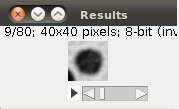
\includegraphics[width=0.75\textwidth]{cropblob.png}  
 % \caption{Difference de Gaussienne (blobs)}
 \end{minipage} \hfill
\begin{minipage}{.450\linewidth}
  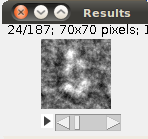
\includegraphics[width=0.5\textwidth]{cropprotDog.png}   
  %\caption{Difference de Gaussienne (protéines)}
 \end{minipage} \hfill
\caption{Exemple d'images formant le \textit{stack} de particules (blobs et protéines)}
\end{center}
\end{figure}

\subsubsection*{Statistiques}

\begin{itemize}
\item[•] La \textbf{Différence de Gaussiennes} permet d'obtenir les résultats suivants :
\end{itemize}

\begin{figure}[!ht]
\begin{center}
 \begin{minipage}{.450\linewidth}
  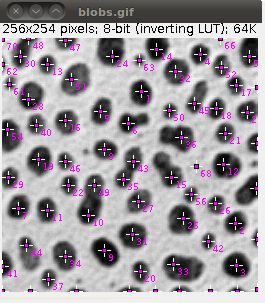
\includegraphics[width=0.75\textwidth]{blobsDog.png}  
 % \caption{Difference de Gaussienne (blobs)}
 \end{minipage} \hfill
\begin{minipage}{.450\linewidth}
  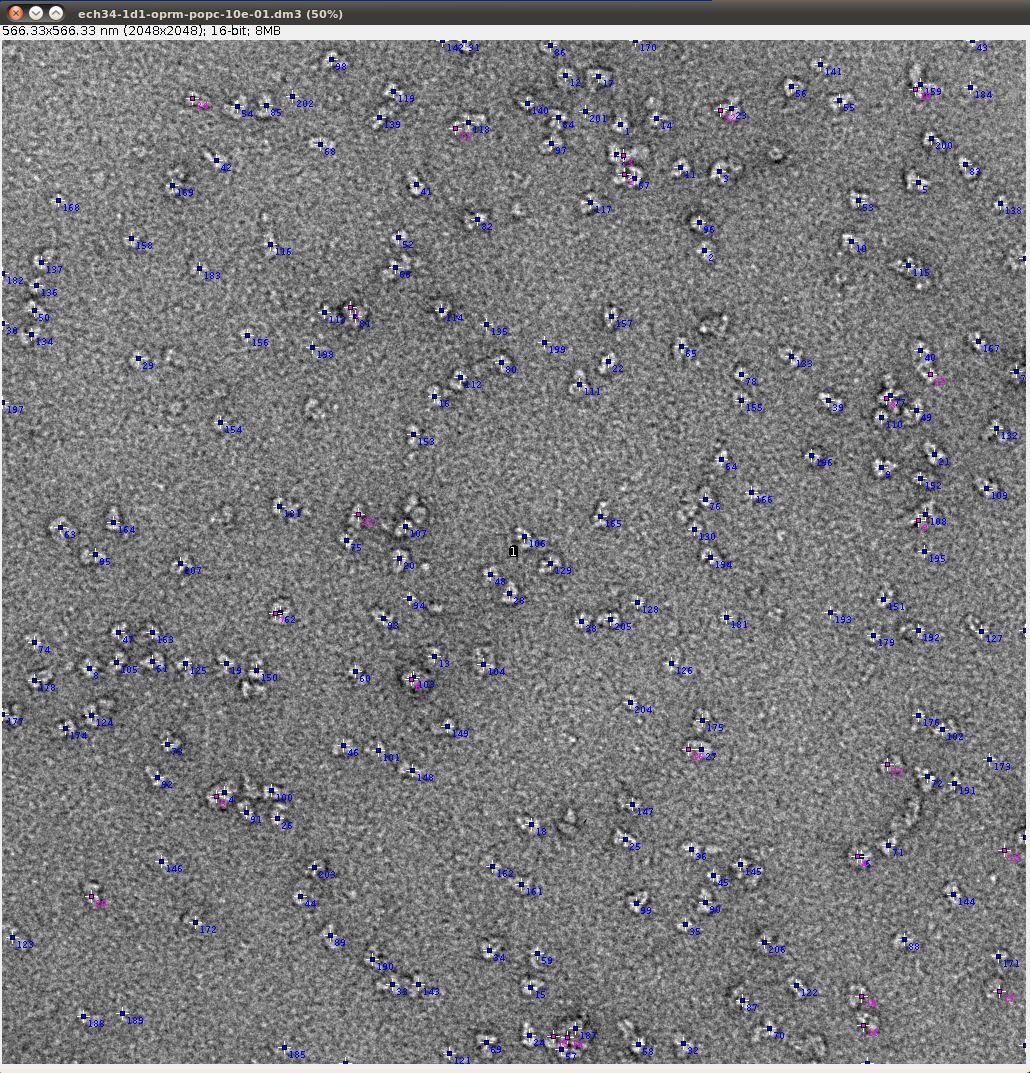
\includegraphics[width=1\textwidth]{protDog.png}   
  %\caption{Difference de Gaussienne (protéines)}
 \end{minipage} \hfill
\caption{Différence de Gaussiennes (blobs et protéines)}
\end{center}
\end{figure}

Nous constatons que ce piquage est efficace sur notre image de protéines membranaires. Nous l'avons également testé sur une image de blobs, qui est une image de référence pour les essais sur \imj , elle semble tout aussi bien marcher. \\

\pagebreak

\begin{itemize}
\item[•] L'\textbf{Extraction de contours} permet d'obtenir les résultats suivants :
\end{itemize}

\begin{figure}[!ht]
\begin{center}
 \begin{minipage}{.450\linewidth}
  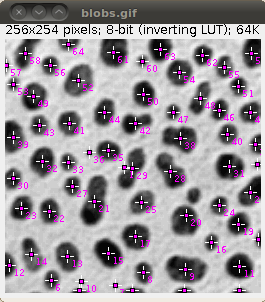
\includegraphics[width=0.75\textwidth]{blobDilate.png}  
 % \caption{Difference de Gaussienne (blobs)}
 \end{minipage} \hfill
\begin{minipage}{.450\linewidth}
  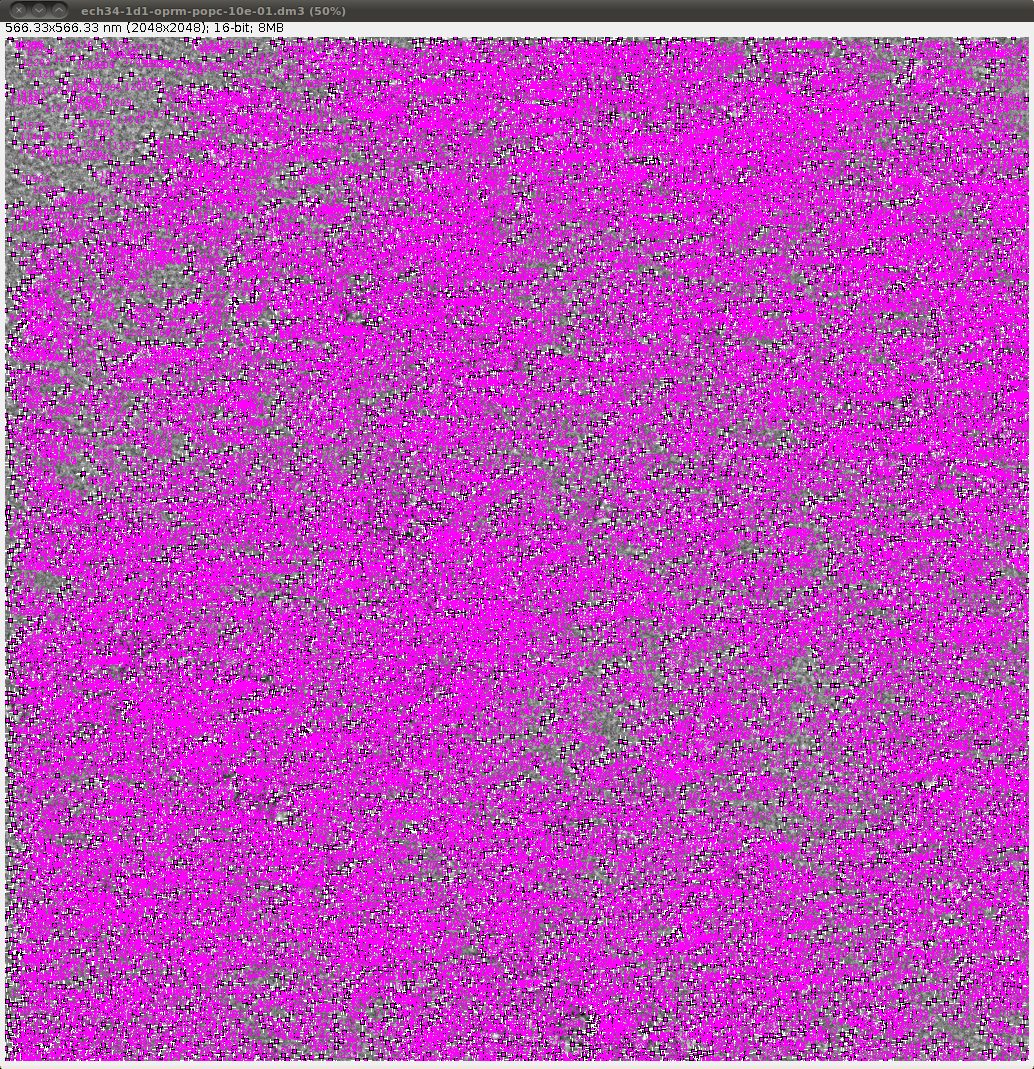
\includegraphics[width=1\textwidth]{protDilate.png}   
  %\caption{Difference de Gaussienne (protéines)}
 \end{minipage} \hfill
\caption{Extraction de contours (blobs et protéines)}
\end{center}
\end{figure}

Nous observons que cet algorithme semble bien fonctionner sur les blobs, alors que sur les protéines il y a beaucoup trop de points de piquage. Même en modifiant le paramètre de la "Noise Tolerance" nous obtenons des résultats de piquage similaires. \\

\begin{itemize}
\item[•] La \textbf{Corrélation d'images} ne permet pas d'obtenir de résultats de piquage exploitables avec ces deux types d'images. Nous avons également testé cet algorithme avec des images de particules virales. Nous obtenions de bon résultats, cependant, pour des raisons de confidentialité, nous ne pouvons pas intégrer ces données dans notre rapport. \\
\end{itemize}

\begin{itemize}
\item[•] \textbf{Résultats} :
\end{itemize}

Nous avons réalisé une série de tests statistiques afin de comparer l'efficacité de nos algorithmes sur les différentes images. Les résultats obtenus sont regroupés dans le tableau (Table \ref{tableau}) suivant :

\begin{table}[h]
\begin{center}
\begin{tabular}{|c|c|c|c|c|}
\hline
\textbf{Images} & \textbf{Variables} & \textbf{DoG} & \textbf{Dilate Difference} & \textbf{Image Correlation} \\
\hline
Blobs & Vrai Positif (VP) & 63 & 61 & null \\
	& Vrai Négatif (VN) & 3 & 0 & null \\
	& Faux Positif (FP) & 9 & 2 & null \\
	& Faux Négatif (FN) & 0 & 1 & null \\
	& Sensibilité (SE) & 1 & 0.98 & null \\
	& Spécificité (SP) & 0.25 & 0 & null \\
\hline
Protéines & Vrai Positif (VP) & 167 & infini & null \\
	& Vrai Négatif (VN) & 8 & infini & null \\
	& Faux Positif (FP) & 16 & infini & null \\
	& Faux Négatif (FN) & 8 & infini & null \\
	& Sensibilité (SE) & 0.95 & null & null \\
	& Spécificité (SP) & 0.5 & null & null \\
	\hline
\end{tabular}
\end{center}
\caption{Tableau de statistiques d'efficacité des algorithmes de piquage}
\label{tableau}
\end{table}

\pagebreak

Les \textbf{Vrais Positifs} sont les particules devant être sélectionnées et qui le sont par l'algorithme. Les \textbf{Vrais Négatifs} représentent tout ce qui ne doit pas être sélectionné et qui ne l'est pas. Les \textbf{Faux Positifs} correspondent à tout ce qui ne doit pas être sélectionné mais qui l'est. Enfin, les \textbf{Faux Négatifs} sont les particules devant être sélectionnées mais qui ne le sont pas. \\ 
La \textbf{Sensibilité}~\cite{stats:url} est la probabilité qu'une particule devant être piquée le soit. Une mesure de la sensibilité s'accompagne toujours d'une mesure de la spécificité. La \textbf{Spécificité} est la probabilité de ne pas sélectionner ce qui ne doit pas l'être. La sensibilité et la spécificité sont obtenues par les formules suivantes : \\

\begin{center}
SE = $\frac{\text{VP}}{\text{VP+FN}}$ et SP = $\frac{\text{VN}}{\text{VN+FP}}$ \\
\end{center}

D'après la Table \ref{tableau}, nous remarquons que c'est l'algorithme de Différence de Gaussiennes qui a la meilleure spécificité et sensibilité pour les blobs. En effet, il y a plus de particules sélectionnées avec ce dernier qu'avec l'Extraction de contours, alors que cet algorithme a été créé pour les blobs au départ. Cependant, nous constatons qu'il y a plus de faux positifs avec la Différence de Gaussiennes. \\
En ce qui concerne les protéines, l'Extraction de contours est inefficace car elle ne fait pas de distinction entre le bruit et les particules. La Différence de Gaussiennes, quant à elle, est assez efficace en ce qui concerne la sélection de ces dernières. 

\section{Ajout d'un nouvel algorithme au plugin}

Voici la marche à suivre pour ajouter un nouvel algorithme de piquage à notre plugin :

\begin{itemize}
\item Ajouter le nom de l'algorithme dans la liste des noms proposés par la \emph{JComboBox} dans la classe \texttt{PickFrame}.
\item Ajouter un nouveau "\textit{case}" dans chaque "\textit{switch}" de la classe \texttt{AlgoFactory}.
\item Créer une nouvelle classe \texttt{PanelAlgorithme} dans laquelle doivent se trouver :
	\begin{itemize}
	\item un \emph{JLabel} pour la phrase d'indication d'utilisation de l'algorithme,
	\item tous les \emph{JLabel}, \emph{JCheckBox}, \emph{JButton}, \emph{JTextField}, \emph{JPanel} nécessaires pour le fonctionnement de l'algorithme,
	\item une méthode \texttt{setAttributes()} pour récupérer les paramètres entrés par l'utilisateur,
	\end{itemize}
\item Créer une nouvelle classe \texttt{Algorithme} pour la procédure de piquage suivant le modèle de ceux déjà implantés. 
\end{itemize}

\section{Améliorations possibles}

Nous avons fait en sorte que notre plugin corresponde le plus possible aux attentes de notre tuteur. Cependant, quelques améliorations restent possibles. \\

Une fonction pour ajouter automatiquement un nouvel algorithme de piquage avec ses paramètres d'entrée via l'interface, sans que l'utilisateur n'ai à toucher au code source, serait pratique. Dans ce cas, il n'y aurait plus qu'à ajouter une classe implémentant cette nouvelle méthode de piquage dans le code. \\

Le mode de création du \textit{stack} d'images individuelles pourrait éviter d'afficher les images dupliquées au cours de la création du \textit{stack}. Cela permettrait d'alléger la mémoire vive de l'ordinateur, ainsi que de diminuer le temps de traitement. \\
De plus, il n'est actuellement pas possible de visualiser les sélections sur toutes les images du \textit{stack} de base en même temps. Il serait donc intéressant de pouvoir le faire. \\

Par ailleurs, le \textit{stack} d'images individuelles peut contenir des éléments qui n'auraient pas dus être sélectionnés ("paquets", bruit de fond). Il serait utile de pouvoir les supprimer du \textit{stack} ou d'ajouter l'image d'une particule n'ayant pas été sélectionnée automatiquement. \\

La gestion de la mémoire pourrait être améliorée en optimisant nos algorithmes (par exemple, en diminuant le nombre d'objets créés lors de l'exécution). \\

Nous avons créé un mode de débogage dans notre interface afin d'aider l'utilisateur si un processus ne se déroule pas correctement. Cependant, ce mode n'est pas encore optimal et pourrait être complété. De plus, nous n'avons pas eu le temps de l'implémenter dans chacun de nos algorithmes. \\

Enfin, il est possible de lancer notre plugin par l'outil Macro d'\imj. Cependant, il subsiste une erreur : la procédure de création du \textit{stack} d'images individuelles se déroule deux fois (une fois sur le \textit{stack} de base et une autre sur le \textit{stack} de particules sélectionnées). Ceci a pour effet d'afficher deux \textit{stacks} finaux au lieu d'un seul. Résoudre ce problème permettrait d'avoir un déroulement optimal de notre programme depuis l'outil Macro. 




















\chapter*{Conclusion}

\addcontentsline{toc}{chapter}{Conclusion}

Le but de notre projet était l'implémentation en \java ~d'un outil pour le logiciel \imj ~permettant un piquage automatique de particules sur des images issues de cryo-microscopie. \\
Notre plugin se présente sous la forme d'une interface et donne à l'utilisateur le choix entre plusieurs algorithmes de piquage. \\
Nous avons implémenté trois algorithmes dans notre plugin : Différence de dilatation, Différence gaussienne et Corrélation d'images. Leur efficacité varie en fonction du type de particule à sélectionner et de la qualité de l'image à traiter. \\

Cette expérience nous a permis de mieux maitriser la programmation en langage \java ~ainsi que de mieux connaitre le fonctionnement du logiciel \imj. De plus, ce premier projet en équipe nous a donné un aperçu plus précis de ce que sera notre futur métier. 


\addcontentsline{toc}{chapter}{Bibliographie}
\bibliographystyle{unsrt}
\bibliography{rapport}

\appendix
\chapter{Annexes}

\addcontentsline{toc}{chapter}{Annexes}

\newpage

\section{Diagramme des classes du plugin Pick\_EM}

\begin{figure}[!ht] 
\begin{center}
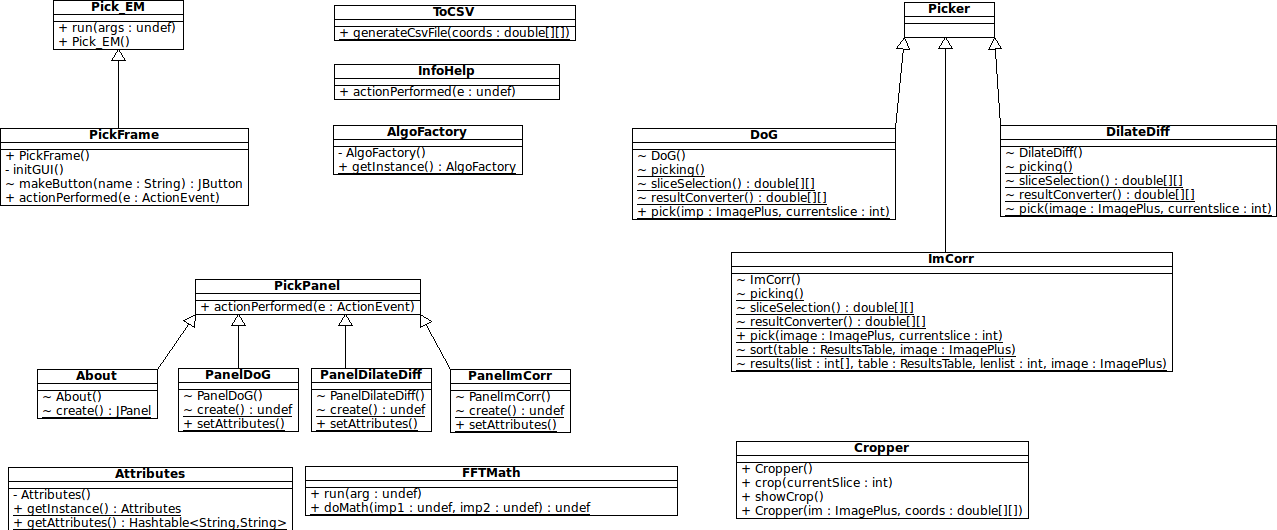
\includegraphics[width=1.4\textwidth, angle=90]{diagComplet.png}
\end{center}
\end{figure}
\section{Code source du plugin ImageJ Pick\_EM}
\end{document}